%%%%%%%%%%%%%%%%%%%%%%%%%%%%%%%%%%%%%%%%%%%%%%%%%%%%%%%%%%%%%%%%%%%%%%
% Lớp 12 | Ứng dụng đạo hàm để khảo sát hàm số | Sự đồng biến và nghịch biến của hàm số
% Dạng 2D1?1-3: Tìm tham số 𝑚 để hàm số đơn điệu
% Số câu: 57  (sinh tự động bởi tach_cau.py; từ nay thầy sửa trực tiếp file này)
%%%%%%%%%%%%%%%%%%%%%%%%%%%%%%%%%%%%%%%%%%%%%%%%%%%%%%%%%%%%%%%%%%%%%%

%%%%%%%%%%%%%%%% TRẮC NGHIỆM 4 PHƯƠNG ÁN %%%%%%%%%%%%%%%%

% nguồn: Phan1_Lop_12_Dai_so_Chuong_1
\begin{ex}%[2D1H1-3]%[ma:5827a2e1]
	 Tìm tất cả các giá trị thực của tham số $ m$ để hàm số $ y=x^3+x^2+mx+1$ đồng biến trên $\left(-\infty;+\infty \right)$.
	\choice 
		{$  m\le\dfrac13$}
		{\True  $ m\ge\dfrac13$}
		 {$ m\ge\dfrac43$}
		 {$ m\le\dfrac43$}
	\loigiai{ 
		Xét  hàm số $ y=x^3+x^2+mx+1$.\\
		Tập xác  định: $\mathscr{D}=\mathbb{R}$ và có đạo hàm $y'=3x^2+2x+m$.\\
		Để hàm số đồng biến trên $\mathbb{R}$ thì $y'\ge0$, $\forall x\in\mathbb{R}$ 
		$\Leftrightarrow\heva{&3>0\\&{\Delta}'={1^2}-3m\le0}$\\ 
		 $\Leftrightarrow m\ge\dfrac13$.
	 }
\end{ex}

% nguồn: Phan1_Lop_12_Dai_so_Chuong_1
\begin{ex}%[2D1H1-3]%[ma:dfd21469]
	Cho hàm số $y=f(x)$ xác định và liên tục trên $\mathbb{R}$ và có bảng biến  thiên như sau
	\begin{center}
		\begin{tikzpicture}
			\tkzTabInit[nocadre = false,lgt = 1,espcl  =3.5]
				 {$x$ /1,$y'$ /1,$y$ /2}{$-\infty$,$2$,$+\infty$}
			\tkzTabLine{,-,$0$,+,} 
			\tkzTabVar{+/ $+\infty$,-/$0$,+/ $+\infty$} 
		\end{tikzpicture}
	\end{center}
	Khẳng định nào sau đây  đúng?
	 \choice
		{Hàm số có $2$ cực  trị}
		{Hàm số có giá trị cực đại bằng $2$} 
		{\True Hàm số có giá trị cực tiểu bằng  $0$}
		{Hàm số có giá trị cực đại tại  $x=0$}
	 \loigiai{Dựa vào bảng biến thiên, ta thấy hàm số đạt cực tiểu tại $x=2$ và $y=0$.\\
	Do đó, giá trị cực tiểu của hàm số bằng $0$.} 
\end{ex}

% nguồn: Phan1_Lop_12_Dai_so_Chuong_1
\begin{ex}%[2D1H1-3]%[ma:1fa189a0]
	Cho hàm số $ y=mx^3+mx^2-(m+1)x+1$. Tìm  tất cả các giá trị của m để hàm số nghịch biến trên $\mathbb{R}$.
	\choice 
		{$\dfrac{-3}4<m<0$} 
		{\True $\dfrac{-3}4\le m\le0$} 
		 {$ m\le0$}
		 {$ m\le\dfrac{-3}4$}
	 \loigiai{
		Ta có $y=mx^3+mx^2-(m+1)x+1\Rightarrow  y'=3mx^2+2mx-m-1$.
		\begin{itemize}
			\item Trường hợp $1$: $ m=0\Rightarrow y'=-1<0$. Hàm số nghịch  biến trên $\mathbb{R}$.\hfill$(1)$
			\item Trường hợp $2$: $ m\ne0$. Hàm số nghịch biến trên $\mathbb{R}$  khi
			\begin{eqnarray*}
				\heva{&a<0\\&\Delta\le0\\} 
				&\Leftrightarrow&\heva{&m<0\\&{{\left(2m\right)}^2}-4.3m.\left(-m-1\right)\le0}\cr 
				 &\Leftrightarrow&\heva{&m<0\\&16{m^2}+12m\le0\\}\cr
				 &\Leftrightarrow&\heva{&m<0\\&\dfrac{-3}4\le m\le0\\}\cr
				&\Leftrightarrow&\dfrac{-3}4\le m<0.\quad(2) 
			\end{eqnarray*}
		\end{itemize}
		Từ $\left(1\right)$ và $(2)$ $\Rightarrow\dfrac{-3}4\le m\le0$. 
	} 
\end{ex}

% nguồn: Phan1_Lop_12_Dai_so_Chuong_1
\begin{ex}%[2D1H1-3]%[ma:ad21d002]
	Cho hàm số $y=\dfrac{mx+2}{2x+m}$, $m$ là tham số thực. Có bao nhiêu giá trị nguyên  của tham số $m$ để hàm số nghịch biến trên từng khoảng xác định.
	 \choice
		{$1$} 
		{\True  $3$}
		{$2$} 
		{$5$} 
	\loigiai{ 
		Tập xác định: $\mathscr{D}=\mathbb{R}\setminus\left\{\dfrac{-m}2\right\}$,  $y'=\dfrac{m^2-4}{(2x+m)^2}$.\\
		Để hàm số nghịch biến trên từng khoảng xác định của nó thì $m^2-4<0\Leftrightarrow-2<m<2$.\\ 
		Do đó có $3$ giá trị  nguyên của tham số $m$ thỏa mãn.
	} 
\end{ex}

% nguồn: Phan1_Lop_12_Dai_so_Chuong_1
\begin{ex}%[2D1H1-3]%[ma:7c236f71]
	Cho hàm số $ f(x)=\dfrac{x-4}{x+m}$. Có bao nhiêu giá trị nguyên âm của tham số $ m$ để hàm số đồng biến  trên từng khoảng xác định.
	 \choice
		 {$4$}
		{$5$} 
		 {\True $3$}
		 {$6$}
	\loigiai{Tập xác định: $\mathscr{D}=\mathbb{R}\setminus\left\{-m\right\}$.\\ 
		 Ta có $y'=\dfrac{m+4}{\left(x+m\right)^2}$.\\
		Hàm số đồng biến trên từng khoảng xác định  $\Leftrightarrow y'>0,\forall x\in\mathscr{D} \Leftrightarrow m+4>0\Leftrightarrow m>-4$.\\
		Vì  $ m$ nguyên âm nên $ m\in\left\{-3;-2;-1\right\}$.\\
		Vậy có $3$  giá trị thỏa mãn.
	 }
\end{ex}

% nguồn: Phan1_Lop_12_Dai_so_Chuong_1
\begin{ex}%[2D1H1-3]%[ma:ca28537d]
	Có bao nhiêu giá trị nguyên dương bé hơn $2024$ của tham số $m$ sao cho hàm số $y = \dfrac{2x^2 +  2x - 1 - 5m}{x - m}$ nghịch biến trên khoảng $(1; 5)$?
	 \choice
		{$2017$} 
		{$2018$} 
		{$2020$} 
		{\True  $2019$}
	 \loigiai{
		Tập xác định $D = \mathbb{R} \setminus \{m\}$ và có $y' = \dfrac{2x^2 - 4mx + 3m + 1}{(x  - m)^2}$.\\
		Hàm số nghịch biến trên khoảng $(1; 5)$ khi  và chỉ khi
		\begin{eqnarray*}
			& & y' = \dfrac{2x^2 - 4mx + 3m + 1}{(x  - m)^2} \le 0,\ \forall x \in (1; 5) \\
			 &\Leftrightarrow& \heva{
			&2x^2 - 4mx + 3m + 1  \le 0,\ \forall x \in (1; 5)\\
			&m  \notin (1; 5)}\\
			 &\Leftrightarrow& \heva{
			&-m +  3 \le 0\\
			&-17m + 51 \le  0\\
			&\hoac{&m \le  1\\&m \ge 5}}\\
			 &\Leftrightarrow& m \ge 5
		\end{eqnarray*}
		Do $m$ nguyên dương, bé hơn $2024$ nên $5 \le m \le  2023$. Vậy có tất cả $2019$ giá trị.
	} 
\end{ex}

% nguồn: Phan1_Lop_12_Dai_so_Chuong_1
\begin{ex}%[2D1H1-3]%[ma:e201fffd]
	Có  bao nhiêu số nguyên $a$ sao cho hàm số $f(x)=x^3+a x^2+3 x+1$ đồng biến trên $\mathbb{R}$?
	 \choice
		 {$0$}
		 {$3$}
		 {$6$}
		{\True $7$} 
	\loigiai{ 
		Ta  có $f'(x)=3x^2+2ax+3$.\\
		Do đó,  hàm số đồng biến trên $\mathbb{R}$ nếu
		$$f'(x) \geq 0  \text {với mọi } x \in \mathbb{R} \Leftrightarrow \Delta^{\prime}=a^2-3\cdot 3 \leq 0 \Leftrightarrow-3 \leq a \leq 3.$$
		\noindent Vậy có $7$ số nguyên $a$ thỏa mãn yêu cầu  là $-3;-2;-1;0;1;2;3$.
	 }
\end{ex}

% nguồn: Phan1_Lop_12_Dai_so_Chuong_1
\begin{ex}%[2D1H1-3]%[ma:0d9699ef]
	Tìm tất cả các giá trị thực của tham số $m$ để hàm số $y=-\dfrac{1}{3}x^3-mx^2+(2m-3)x-m+2$  nghịch biến trên $\mathbb{R}$.
	\choice 
		{$m\le -3$, $m\ge  1$}
		 {$-3<m<1$}
		 {\True $-3\le m\le 1$}
		 {$m\le 1$}
	\loigiai{ 
		Ta có  $y'=-x^2-2mx+(2m-3)$.\\
		Hàm số  nghịch biến trên $\mathbb{R}$ khi
		\begin{align*}
			 &~ y'\le 0 , \forall x\in\mathbb{R}\\
			\Leftrightarrow &~ \heva{&a=-1<0\\& \Delta' \le  0} \\
			\Leftrightarrow  &~ m^2+2m-3\le 0 \\
			\Leftrightarrow  &~-3\le m \le 1.
		\end{align*}
	} 
\end{ex}

% nguồn: Phan1_Lop_12_Dai_so_Chuong_1
\begin{ex}%[2D1H1-3]%[ma:328be2ef]
	Có bao nhiêu giá trị nguyên của tham số $m$ để hàm số $y=\dfrac{x+m^2}{x+4}$ đồng biến trên từng khoảng xác định  của nó?
	 \choice
		 {$5$}
		{$1$} 
		 {$2$}
		{\True $3$} 
	 \loigiai{
		Tập xác định: $D=\mathbb{R}\setminus \{-4\}$. Khi  đó ta có: $ y'=\dfrac{4-m^2}{(x+4)^2}$.\\
		Hàm số $y=\dfrac{x+m^2}{x+4}$ đồng biến trên từng khoảng xác định của nó khi và chỉ khi\\ 
		\[y'  > 0,\forall x\ne-4\Leftrightarrow 4-m^2 > 0\Leftrightarrow-2< m < 2.\]
		Theo đề bài, $m\in \mathbb{Z}$ nên $m\in  \{-1;0;1\}$.
	} 
\end{ex}

% nguồn: Phan1_Lop_12_Dai_so_Chuong_1
\begin{ex}%[2D1H1-3]%[ma:c3c6a51f]
	Có bao nhiêu giá trị nguyên dương của tham số $m$ sao cho hàm số $y = \dfrac{2x^2 + (1 - m)x  + 1 + m}{x - m}$ đồng biến trên khoảng $(1; +\infty)$?
	 \choice
		{$3$} 
		 {$1$}
		{$2$} 
		{\True  $0$}
	 \loigiai{
		Tập xác định $D = \mathbb{R} \setminus \{m\}$. Ta có $y' = \dfrac{2x^2 - 4mx + m^2 - 2m -  1}{(x - m)^2} = \dfrac{g(x)}{(x - m)^2}$.\\
		Hàm số đồng biến trên $(1; +\infty)$ khi và chỉ khi $g(x) \ge 0,\  \forall x > 1$ và $m \le 1$.\\
		Vì $\Delta'_g = 2(m + 1)^2 \ge 0,\ \forall m$ nên $g(x) = 0$ có hai nghiệm  thỏa $x_1 \le x_2 \le 1$.\\
		Điều kiện tương đương  là
		 \[
		 \heva{
		&2g(1) = 2(m^2  - 6m + 1) \ge 0\\
		&m \le  1
		} 
		\Leftrightarrow m \le 3 - 2\sqrt{2} \approx  0{,}2.
		\] 
		Do đó không có giá trị  nguyên dương của $m$ thỏa yêu cầu bài toán.
	} 
\end{ex}

% nguồn: Phan1_Lop_12_Dai_so_Chuong_1
\begin{ex}%[2D1H1-3]%[ma:e453d3d6]
	Cho  hàm số $y=f(x)$ có bảng biến thiên như sau
	\begin{center}
		\begin{tikzpicture}
			\tkzTabInit[nocadre = false,lgt  = 1,espcl = 3]
				 {$x$ /1,$y'$ /1,$y$ /2}{$-\infty$,$0$,$2$,$+\infty$}
			 \tkzTabLine{,+,$0$,-,$0$,+,}
			\tkzTabVar{-/ $-\infty$,+/ $3$,-/ $0$,+/  $+\infty$}
		\end{tikzpicture}
	\end{center}
	Tìm giá  trị cực đại $y_{\text{ CĐ}}$ và giá trị cực tiểu $y_{\text{ CT}}$ của hàm số đã cho.
	 \choice
		 {$y_{\text{ CĐ}}=3$ và $y_{\text{ CT}}=2$}
		{$y_{\text{ CĐ}}=2$ và $y_{\text{  CT}}=0$}
		 {$y_{\text{ CĐ}}=3$ và $y_{\text{ CT}}=3$}
		{\True $y_{\text{ CĐ}}=3$  và $y_{\text{ CT}}=0$}
	\loigiai{ 
		Dựa vào bảng biến  thiên ta có $y_{\text{ CĐ}}=3$ và $y_{\text{ CT}}=0$.
	} 
\end{ex}

% nguồn: Phan1_Lop_12_Dai_so_Chuong_1
\begin{ex}%[2D1H1-3]%[ma:e66cba50]
	Số  giá trị nguyên của tham số $ m$ để hàm số $ y=(m^2-1)x^3+(m-1)x^2-x$ nghịch biến trên $\mathbb{R}$ là
	\choice 
		{\True $2$} 
		 {$3$}
		 {$1$}
		{$0$} 
	\loigiai{ 
		Yêu cầu đề bài tương đương với $y'=3(m^2-1)x^2+2(m-1)x-1\le0$, $\forall x\in\mathbb{R}$.\\ 
		\begin{itemize}
			\item Khi  $m^2-1=0\Leftrightarrow m=\pm1$.
			\begin{itemize}
				\item Với $ m=1$ thì  $y'=-1<0$, $\forall x\in\mathbb{R}$ do đó giá trị $ m=1$ thỏa mãn.
				\item Với $ m=-1$ thì $y'=-4x-1\le0\Leftrightarrow x\ge-\dfrac14$, do đó giá trị $ m=-1$ không thỏa mãn. 
			\end{itemize}
			\item Khi $m^2-1\ne0\Leftrightarrow m\ne\pm1$, YCBT tương đương với 
			\begin{eqnarray*}
				&&\heva{&m^2-1<0\\&(m-1)^2+3(m^2-1)\le0}\\ 
				&\Leftrightarrow&\heva{&-1<m<1\\&-\dfrac12\le  m\le1}\\
				 &\Leftrightarrow&-\dfrac12\le m<1.
			\end{eqnarray*}
		\end{itemize}
		Vậy $-\dfrac12\le m\le1$ nên có $2$ giá trị nguyên của tham số $ m$ là $  m=0$; $m=1$ thoả mãn.
	 }
\end{ex}

% nguồn: Phan1_Lop_12_Dai_so_Chuong_1
\begin{ex}%[2D1H1-3]%[ma:6d07edea]
	Cho hàm số $y=f(x)$ có bảng biến thiên  như sau.
	Mệnh đề nào  dưới đây là \textbf{sai?}
	\begin{center}
		\begin{tikzpicture}
			 \tkzTabInit[nocadre = false,lgt = 1,espcl = 3]
				{$x$  /1,$y'$ /1,$y$ /2}{$-\infty$,$0$,$2$,$+\infty$}
			\tkzTabLine{,+,$0$,-,$0$,+,} 
			 \tkzTabVar{-/ $-\infty$,+/ $3$,-/ $0$,+/ $+\infty$}
		\end{tikzpicture}
	\end{center}
	\choice 
		{\True Hàm số \textbf{không}  đạt cực tiểu tại điểm $x=2$}
		{Hàm số  đạt cực đại tại điểm $x=0$}
		{Giá trị cực đại của hàm số là $y=3$} 
		{Giá trị cực  tiểu của hàm số là $y=0$}
	\loigiai{Hàm số đạt cực  tiểu tại điểm $x=2$.}
\end{ex}

% nguồn: Phan1_Lop_12_Dai_so_Chuong_1
\begin{ex}%[2D1H1-3]%[ma:e33c5225]
	Tìm tất cả giá trị của $ m$ sao cho hàm số $ y=\dfrac{x+m}{x+2}$ đồng biến trên các khoảng xác  định?
	\choice 
		{$  m\ge2$}
		{\True $  m<2$}
		 {$ m\le2$}
		{$ m>2$} 
	\loigiai{ 
		Hàm số $ y=\dfrac{x+m}{x+2}$ đồng  biến trên các khoảng xác định khi
		\begin{center}
			$y'=\dfrac{2-m}{(x+2)^2}>0$, $\forall x\ne-2\Leftrightarrow 2-m>0\Leftrightarrow m<2$. 
		\end{center}
	} 
\end{ex}

% nguồn: Phan1_Lop_12_Dai_so_Chuong_1
\begin{ex}%[2D1H1-3]%[ma:8b41acff]
	Số giá trị nguyên của $ m$ để  hàm số $ y=(m-7)x^3+(m-7)x^2-2mx-1$ nghịch biến trên $\mathbb{R}$ bằng
	\choice 
		{\True $7$} 
		{$9$} 
		 {$4$}
		 {$6$}
	 \loigiai{
		Tập  xác định: $\mathscr{D}=\mathbb{R}$.\\
		 Ta có $y'=3(m-7)x^2+2(m-7)x-2m$.
		\begin{itemize}
			\item Trường  hợp $1$: $ m=7\Rightarrow y'=-14<0$, $\forall x\in\mathbb{R}\Rightarrow$ hàm số nghịch biến trên $\mathbb{R}$ $\Rightarrow m=7$.
			\item Trường hợp $2$: $ m\ne 7$.\\ 
			Hàm số nghịch biến trên $\mathbb{R}$ $\Leftrightarrow y'\le0$, $\forall  x\in\mathbb{R}$
			\begin{eqnarray*}
				 &\Leftrightarrow&\heva{&m-7<0\\&{\Delta}'\le0}\\
				 &\Leftrightarrow&\heva{&m<7\\&7{m^2}-56m+49\le0}\\
				&\Leftrightarrow&\heva{&m<7\\&1\le  m\le7}\\
				 &\Leftrightarrow&1\le m<7.
			\end{eqnarray*}
		\end{itemize}
		Vậy hàm số nghịch  biến trên $\mathbb{R}$ khi $1\le m\le7$. Do $ m\in\mathbb{Z}$ nên có $7$ giá trị nguyên của $ m$.
	 }
\end{ex}

% nguồn: Phan1_Lop_12_Dai_so_Chuong_1
\begin{ex}%[2D1V1-3]%[ma:c21531ca]
	Tìm giá trị lớn nhất của tham số $m$ để hàm số $y=\dfrac{1}{3}x^3-mx^2+(8-2m)x+m+3$ đồng  biến trên $\mathbb{R}$.
	\choice 
		{$m=-4$} 
		 {$m=-2$}
		{$m=4$} 
		 {\True $m=2$}
	 \loigiai{
		Tập xác định $D=\mathbb{R}$ và có đạo hàm $y'=x^2-2mx+8-2m$.\\ 
		Hàm số đồng  biến trên $\mathbb{R}$
		$\Leftrightarrow y'\ge 0$, $\forall x\in \mathbb{R}$ 
		\allowdisplaybreaks 
		\begin{eqnarray*}
			&\Leftrightarrow& x^2-2mx+8-2m\ge 0, \forall x\in  \mathbb{R}\\
			&\Leftrightarrow& \heva{&  a > 0\\
			& \Delta '\le  0
			 }\\
			&\Leftrightarrow& \heva{& 1> 0\\ 
			& m^2+2m-8\le  0\\
			 }\\
			&\Leftrightarrow&-4\le  m\le 2.
		\end{eqnarray*}
		Giá trị lớn nhất của  tham số $m$ để hàm số $y=\dfrac{1}{3}x^3-mx^2+(8-2m)x+m+3$ đồng biến trên $\mathbb{R}$ là $m=2$.
	} 
\end{ex}

% nguồn: Phan1_Lop_12_Dai_so_Chuong_1
\begin{ex}%[2D1V1-3]%[ma:6061ad11]
	 Có bao nhiêu giá trị nguyên âm của tham số $m$ để hàm số $y=x+3-\dfrac{m}{x-2}$ đồng biến trên $[5;+\infty)$?
	 \choice
		 {$3$}
		{$2$} 
		{$8$} 
		{\True $9$} 
	 \loigiai{
		Điều kiện xác  định: $x\ne 2$.\\
		Ta có: $y'=1+\dfrac{m}{(x-2)^2}$.\\ 
		Hàm số $y$ đồng biến trên $[5;+\infty) \Leftrightarrow  y'\ge 0,\forall x\in [5;+\infty)$
		 \allowdisplaybreaks
		\begin{eqnarray*}
			&\Leftrightarrow& 1+\dfrac{m}{(x-2)^2}\ge 0, \forall  x\in [5;+\infty)\\
			 &\Leftrightarrow& m\ge-(x-2)^2, \forall x\in [5;+\infty)\\
			&\Leftrightarrow& m\ge \max\limits_{[5;+\infty)}\left[-(x-2)^2\right].\quad (*) 
		\end{eqnarray*}
		Đặt $g(x)=-(x-2)^2$, ta có $g'(x)=-2(x-2) < 0,\forall  x\in [5;+\infty)$.
		\begin{center}
			\begin{tikzpicture}
				\tkzTabInit 
					[lgt=2,espcl=0.02\linewidth] 
					{$x$/.8,$f’(x)$/.8,$f (x)$/2} 
					{$-5$,$+\infty$} 
				 \tkzTabLine{,-,}
				 \tkzTabVar{+/ $-9$,-/ $-\infty$}
			\end{tikzpicture}
		\end{center}
		Khi đó (*) $\Leftrightarrow m\ge-9$. Vì $m$  nguyên âm nên $m\in \{-9;-8;-7;\ldots;-1\}$.\\
		Vậy có $9$ giá trị  $m$ cần tìm.
	} 
\end{ex}

% nguồn: Phan1_Lop_12_Dai_so_Chuong_1
\begin{ex}%[2D1V1-3]%[ma:5b636e1e]
	Tập tất cả các giá trị thực của tham số $m$ để hàm số $y=-\dfrac{1}{3}x^3-mx^2+(2m-3)x-m+2$  luôn nghịch biến trên $\mathbb{R}$ là $m\in [a;b]$. Giá trị $b-a$ bằng.
	\choice 
		 {\True $4$}
		{$10$} 
		 {$12$}
		 {$-3$}
	 \loigiai{
		Ta  có: $y'=-x^2-2mx+2m-3$.\\
		Để hàm số nghịch biến trên $\mathbb{R}$ thì 
		$\heva{&  a < 0\\
		 & \Delta \le 0
		}$ 
		\begin{eqnarray*}
			&\Rightarrow& \heva{&-1< 0\\& m^2-(-1)(2m-3)\le 0}\\ 
			&\Leftrightarrow& m^2+2m-3\le 0\\ 
			&\Leftrightarrow& -3\le m\le  1.
		\end{eqnarray*}
		Suy  ra $a=-3$; $b=1\Rightarrow b-a=1-(-3)=4$.
	} 
\end{ex}

% nguồn: Phan1_Lop_12_Dai_so_Chuong_1
\begin{ex}%[2D1V1-3]%[ma:4270a009]
	Tìm tất cả các giá trị của  tham số $m$ để hàm số $ y=\sqrt3\sin x+\cos x-mx+5$ nghịch biến trên tập xác định.
	\choice 
		 {\True $ m\ge2$}
		{$  m\le2$}
		 {$ m\ge-2$}
		{$-2\le  m\le2$}
	 \loigiai{
		Tập xác định $\mathscr{D}=\mathbb{R}$ và có đạo hàm $y'=\sqrt3\cos x-\sin  x-m$.\\
		Hàm số $ y=\sqrt3\sin x+\cos x-mx+5$ nghịch biến trên  $\mathbb{R}$
		\begin{align*}
			 &\Leftrightarrow y'=\sqrt3\cos x-\sin x-m\le0,\ \forall x\in\mathbb{R}\cr
			&\Leftrightarrow\dfrac{\sqrt3}2\cos x-\dfrac12\sin x\le\dfrac m2,\  \forall x\in\mathbb{R}\cr
			 &\Leftrightarrow\sin\left(x-\dfrac{\pi }3\right)\le\dfrac m2,\forall x\in\mathbb{R}.&(2)
		\end{align*}
		Vì $-1\le\sin\left(x-\dfrac{\pi }3\right)\le1$,  $\forall x\in\mathbb{R}$ nên $(2)\Leftrightarrow\dfrac m2\ge1\Leftrightarrow m\ge2$.
	 }
\end{ex}

% nguồn: Phan1_Lop_12_Dai_so_Chuong_1
\begin{ex}%[2D1V1-3]%[ma:b59ca3f0]
	Cho hàm số $y=\dfrac{\left(m+1\right)x+2m+2}{x+m}$. Với giá trị  nào của $m$ thì hàm số nghịch biến trên $\left(-1;+\infty \right)$?
	 \choice
		{$m < 1$} 
		{$1\le  m < 2$}
		 {$\hoac{&m<1\\
		 &m>2}$}
		 {\True $m > 2$}
	\loigiai{Tập xác định: $D=\mathbb{R}\setminus \{-m\}$ có đạo hàm $y'=\dfrac{\left(m+1\right)m-\left(2m+2\right)}{\left(x+m\right)^2}=\dfrac{m^2-m-2}{\left(x+m\right)^2}$, $\forall x \ne-m$.\\ 
		Hàm số đồng biến trên  $\left(-1;+\infty \right)$ khi và chỉ khi $$\heva{&{-m\notin \left(-1;+\infty \right)} \\
		&{m^2-m-2> 0} 
		} \Leftrightarrow \heva{&{-m\le-1} \\ 
		&{\hoac{&{m > 2}  \\
		 &{m <-1}
		 }
		}} \Leftrightarrow m >  2.$$
	 }
\end{ex}

% nguồn: Phan1_Lop_12_Dai_so_Chuong_1
\begin{ex}%[2D1V1-3]%[ma:f4f6961f]
	Cho hàm số $y=\dfrac{mx+2m+3}{x+m}$ với $m$ là tham số thực. Gọi $S$ là tập hợp tất cả các giá trị nguyên của $m$ để hàm  số nghịch biến trên khoảng $\left(2;+\infty \right)$. Tìm số phần tử của $S$.
	\choice 
		{$4$} 
		 {$2$}
		{$5$} 
		 {\True $3$}
	\loigiai{ 
		Ta có: $y=\dfrac{mx+2m+3}{x+m} \Rightarrow y'=\dfrac{m^2-\left(2m+3\right)}{\left(x+m\right)^2}=\dfrac{m^2-2m-3}{\left(x+m\right)^2}$, $\forall x \ne-m$.\\ 
		Hàm số đã cho nghịch biến trên khoảng $\left(2;+\infty \right)$ khi và chỉ khi $$y' < 0, \forall x\in \left(2;+\infty  \right)
		\Leftrightarrow \heva{&{m^2-2m-3<  0} \\
		&{-m\le  2}
		} \Leftrightarrow \heva{&{-1< m <  3} \\
		&{m\ge-2} 
		} \Leftrightarrow-1<  m < 3.$$
		Vì $m\in \mathbb{Z}$ nên $m\in \left\{0,1, 2\right\}$, suy ra $S=\left\{0,1, 2\right\}$ nên $S$ có $3$ phần  tử.
	} 
\end{ex}

% nguồn: Phan1_Lop_12_Dai_so_Chuong_1
\begin{ex}%[2D1V1-3]%[ma:6f645881]
	Tổng các giá trị nguyên âm của $m$ để hàm số $y=x^3+mx-\dfrac{1}{5x^5}$  đồng biến trên khoảng $\left(0;+\infty \right)$ là
	\choice 
		{\True $-10$} 
		 {$-3$}
		{$-6$} 
		 {$-7$}
	 \loigiai{
		Hàm số đồng biến trên khoảng $(0;+\infty)$ $\Leftrightarrow y'=3x^2+m+\dfrac{1}{x^6} \ge 0$ với $\forall  x\in \left(0;+\infty \right) \left(*\right)$.\\
		Theo bất đẳng thức Cauchy, với $ \forall x\in \left(0;+\infty \right)$  ta có
		 $$y'=3x^2+\dfrac{1}{x^6}+m=\left(x^2+x^2+x^2+\dfrac{1}{x^6} \right)+m\ge 4\sqrt[4]{x^2.x^2.x^2.\dfrac{1}{x^6}}+m=4+m.$$
		Để hàm số đồng biến trên khoảng $(0;+\infty)$ thì 
		$$ \left(*\right)\Leftrightarrow m+4\ge 0\Leftrightarrow m\ge-4 .$$ 
		 Vì $m$ nguyên âm nên $m\in \left\{-4;-3;-2;-1\right\}$. Vậy tổng các giá trị của $m$ là $-10$.
	 }
\end{ex}

% nguồn: Phan1_Lop_12_Dai_so_Chuong_1
\begin{ex}%[2D1V1-3]%[ma:918c609a]
	Cho hàm số $y=\dfrac{mx-2m-3}{x-m}$ với $m$ là tham  số. Gọi $S$ là tập hợp tất cả các giá trị nguyên của $m$ để hàm số đồng biến trên khoảng $\left(2;+\infty \right)$. Tìm số phần tử của $S$.
	 \choice
		{$1$} 
		 {$5$}
		 {$4$}
		{\True  $3$}
	\loigiai{ 
		Điều  kiện xác định: $x\ne m$.\\
		Ta có $y'=\dfrac{-m^2+2m+3}{\left(x-m\right)^2}$, $\forall  x \ne m$.\\
		Hàm số đã cho đồng biến trên  khoảng $\left(2;+\infty \right)$ khi và chỉ khi
		\allowdisplaybreaks 
		\begin{eqnarray*}
			&&\heva{&{y'=\dfrac{-m^2+2m+3}{\left(x-m\right)^2} > 0, \quad \forall x  > 2} \\
			&{m\notin  \left(2;+\infty \right)}
			 } \\
			&\Leftrightarrow& \heva{&{-m^2+2m+3> 0} \\ 
			&{m\le 2} 
			}\\ &\Leftrightarrow &\heva{&{-1< m < 3} \\ 
			 &{m\le 2}
			} \\ &\Leftrightarrow&-1< m\le  2.
		\end{eqnarray*}
		Suy ra $S=\left\{0;1;2\right\}$.  Vậy số phần tử của $S$ là $3$.
	} 
\end{ex}

% nguồn: Phan1_Lop_12_Dai_so_Chuong_1
\begin{ex}%[2D1V1-3]%[ma:5553109e]
	Có bao nhiêu giá trị nguyên của tham số $m$ thuộc đoạn $\left[1;\,20 \right]$ để ứng với mỗi, hàm số $y=\dfrac{-x^2+3x-m-1}{3x-m}$ đồng biến trên khoảng  $\left( 2;\,3 \right)$?
	 \choice
		 {$17$}
		 {$14$}
		 {\True $15$}
		{$13$} 
	 \loigiai{
		 Điều kiện: $x\ne \dfrac{m}{3}$ có đạo hàm $y'=\dfrac{-3x^2+2mx+3}{\left( 3x-m \right)^2} $.\\
		Hàm số $y=\dfrac{-x^2+3x-m-1}{3x-m}$ đồng biến  trên khoảng $\left( 2;\,3 \right)$ khi và chỉ khi
		$$\dfrac{-3x^2+2mx+3}{\left(3x-m\right)^2}  \ge 0;\forall x \in \left( 2;3 \right) \Leftrightarrow \heva{
		& -3x^2+2mx+3\ge 0;\text{  }\forall x\in \left( 2;3 \right)\text{ }&\left( 1 \right) \\
		& \dfrac{m}{3} \notin \left( 2;\,3 \right).&\left( 2 \right) 
		 }$$
		Ta có $\left( 2 \right)\Leftrightarrow  \hoac{
		&  \dfrac{m}{3}\ge 3 \\
		&  \dfrac{m}{3}\le 2 }\Leftrightarrow \hoac{
		 & m\ge 9 \\
		& m\le 6 } $ . Khi đó $\left( 1 \right)\Leftrightarrow 2m\ge 3x-\dfrac{3}{x}=g(x)$,$\forall x\in \left(  2;3 \right)$.\\
		Mà $g'(x)=3+\dfrac{3}{x^2}>0$,$\forall x\in \left( 2;3 \right)\Rightarrow g(x) $ luôn đồng biến trên $\left(  2;3 \right)$.\\
		Do đó $2m\ge 3x-\dfrac{3}{x}=g(x),\forall x\in \left( 2;3 \right) \Leftrightarrow 2m\ge g(3) \Leftrightarrow 2m\ge 8\Leftrightarrow m\ge 4$.\\ 
		Kết hợp với (2) ta được $  \hoac{
		& m\ge 9  \\
		& 4\le m\le  6 \\
		} $.\\ Vì $m\in \mathbb{Z}$ nên $m\in \left\{4;\,5;\,6;\,9;\,10;...;\,20 \right\}$.\\ 
		 Vậy có $15$ số nguyên $m$ thỏa mãn.
	 }
\end{ex}

% nguồn: Phan1_Lop_12_Dai_so_Chuong_1
\begin{ex}%[2D1V1-3]%[ma:b2c33c7d]
	Có bao nhiêu giá trị nguyên dương không lớn hơn 2024  của tham số $m$ sao cho hàm số $y=\dfrac{x^2+2x-1+m}{5x+m}$ nghịch biến trên khoảng $\left( -3;1 \right)$?
	 \choice
		{$2012$} 
		{$2009$} 
		 {$2011$}
		{\True $2010$} 
	 \loigiai{
		Tập xác định  $D=\mathbb{R} \setminus \left\{-\dfrac{m}{5} \right\}$ và có đạo hàm $y'=\dfrac{5x^2+2mx-3m+1}{\left(5x+m\right)^2}$.\\
		Hàm số nghịch biến  trên khoảng $\left( -3;1 \right)$ khi và chỉ khi
		$y'=\dfrac{5x^2+2mx-3m+1}{\left(5x+m\right)^2} \le 0 ,\forall x \in  \left( -3;1 \right)$.\\
		$\Leftrightarrow  \heva{
		& 5x^2+2mx-3m+1 \le 0,\forall x\in \left( -3;1  \right) \\
		& -\dfrac{m}{5}\notin \left( -3;1 \right)  } \Leftrightarrow \heva{
		 & -9m+46\le 0 \\
		& -m+6\le  0 \\
		& \hoac{ 
		& m\le -5 \\ 
		& m\ge  15\\
		} } 
		\Leftrightarrow  \heva{
		& m\ge \dfrac{46}{9}  \\
		 & m\ge 6 \\
		& \hoac{ 
		 & m\le -5 \\
		 & m\ge 15 \\
		 }}
		\Leftrightarrow m\ge  15 \\
		$.\\ 
		Do m  nguyên dương và không lớn hơn $2024$ nên $15\le m\le 2024$.\\
		Vậy có tất  cả $2010$ giá trị.
	 }
\end{ex}

% nguồn: Phan1_Lop_12_Dai_so_Chuong_1
\begin{ex}%[2D1V1-3]%[ma:e9ca3a0b]
	Có bao nhiêu giá trị nguyên của tham số $m$ để  hàm số $y=\dfrac{x^2+2x+m}{x-1}$ nghịch biến trên khoảng $\left( 1;3 \right)$ và đồng biến trên khoảng $\left( 4;6 \right)$.
	 \choice
		 {$6$}
		 {$7$}
		 {$5$}
		{\True  $4$}
	 \loigiai{
		Ta có  ${y}'=\dfrac{x^2-2x-2-m}{(x-1)^2}$.\\
		Hàm số nghịch biến trên khoảng $\left( 1;\,3 \right)$ và đồng biến trên khoảng $\left( 4;\,6 \right)$ khi và chỉ  khi\\ $\heva{
		& {y}'\le 0,\forall  x\in \left( 1;\,3 \right) \\
		& {y}'\ge  0,\forall x\in \left( 4;\,6 \right) \\
		} \Leftrightarrow  \heva{
		& x^2-2x-2-m\le 0,\forall x\in \left( 1;3 \right) \\ 
		&  x^2-2x-2-m\ge 0,\forall x\in \left( 4;\,6 \right)
		}  \Leftrightarrow \heva{
		& m\ge x^2-2x-2,\forall  x\in \left( 1;3 \right) \\
		& m\le x^2-2x-2,\forall x\in \left( 4;\,6  \right)
		 }$\\
		Xét hàm  số $g(x)=x^2-2x-2,\,\,g'(x)=2x-2$ ta có bảng biến thiên của $g(x)$ như sau
		\begin{center}
			\begin{tikzpicture}[scale=0.7,line join=round,>=stealth]
				\def\myltespcl{3}\def\myltlgt{2}\def\myltdeltacl{0.5} 
				 \def\myltx{0.7}\def\mylta{0.7}\def\myltb{3.5}\def\myltc{\myltb/5}
				\path  (\myltlgt/2,-\myltx/2) node {$x$}
					(\myltlgt/2,-\myltx-\mylta/2) node {$y'$} 
					(\myltlgt/2,-\myltx-\mylta-\myltb/2) node  {$y$};
				\draw (0,-\myltx)--(\myltlgt+5*\myltespcl+2*\myltdeltacl,-\myltx) 
					(0,-\myltx-\mylta)--(\myltlgt+5*\myltespcl+2*\myltdeltacl,-\myltx-\mylta) 
					 (\myltlgt,0)--(\myltlgt,-\myltx-\mylta-\myltb);
				\path (\myltlgt+\myltdeltacl,-\myltx/2)  node {$-\infty$};
				\path  (\myltlgt+\myltdeltacl+0.5*\myltespcl,-\myltx-\mylta/2) node {$-$};
				\path (\myltlgt+\myltdeltacl+\myltespcl,-\myltx/2) node {$1$}; 
				\path (\myltlgt+\myltdeltacl+2*\myltespcl,-\myltx/2) node  {$3$};
				\path (\myltlgt+\myltdeltacl+3*\myltespcl,-\myltx/2)  node {$4$};
				\path (\myltlgt+\myltdeltacl+3.5*\myltespcl,-\myltx-\mylta/2) node  {$+$};
				 \path (\myltlgt+\myltdeltacl+4*\myltespcl,-\myltx/2) node {$6$};
				\path (\myltlgt+\myltdeltacl+5*\myltespcl,-\myltx/2)  node {$+\infty$};
				\path (\myltlgt+\myltdeltacl+\myltespcl,-\myltx-\mylta/2)  node {$0$};
				 \node (nmylta) at (\myltlgt+\myltdeltacl,-\myltx-\mylta-0.5*\myltc) {$+\infty$};
				\node  (nmyltb) at (\myltlgt+\myltdeltacl+\myltespcl,-\myltx-\mylta-4.5*\myltc) {$-3$};
				\node  (nmyltc) at (\myltlgt+\myltdeltacl+2*\myltespcl,-\myltx-\mylta-3.5*\myltc) {$3$};
				 \node (nmyltd) at (\myltlgt+\myltdeltacl+3*\myltespcl,-\myltx-\mylta-2.5*\myltc) {$6$};
				\node (nmylte) at (\myltlgt+\myltdeltacl+4*\myltespcl,-\myltx-\mylta-1.5*\myltc) {$18$}; 
				\node (nmyltf) at (\myltlgt+\myltdeltacl+5*\myltespcl,-\myltx-\mylta-0.5*\myltc) {$+\infty$}; 
				\draw[->] (nmylta)--(nmyltb); 
				 \draw[->] (nmyltb)--(nmyltc);
				\draw[->]  (nmyltc)--(nmyltd);
				\draw[->] (nmyltd)--(nmylte); 
				\draw[->]  (nmylte)--(nmyltf);
			\end{tikzpicture}
		\end{center}
		Từ bảng biến thiên của $g(x)$ ta có $\left( * \right)\Leftrightarrow 3\le  m\le 6$.\\
		Vì  $m$ là số nguyên nên chọn $m\in \left\{3;4;5;6 \right\}$.\\
		Vậy có $4$ giá trị nguyên của $m$ thỏa mãn  bài toán.
	} 
\end{ex}

% nguồn: Phan1_Lop_12_Dai_so_Chuong_1
\begin{ex}%[2D1V1-3]%[ma:99769a38]
	Có tất cả bao  nhiêu số nguyên dương $m$ để hàm số $y=\dfrac{\cos x+1}{10\cos x+m}$ đồng biến trên khoảng $\left(0;\dfrac{\pi}{2} \right)$.
	 \choice
		 {\True $9$}
		 {$8$}
		{$10$} 
		{$11$} 
	\loigiai{Đặt $t=\cos x$, $\left(0< t < 1\right)$ ta có $y=\dfrac{t+1}{10t+m} \Rightarrow y'=\dfrac{m-10}{\left(10t+m\right)^2}\cdot t'$.\\ 
		Hàm số $y=\dfrac{\cos x+1}{10\cos x+m}$ đồng biến trên khoảng $\left(0;\dfrac{\pi}{2} \right)$ khi và chỉ khi $$y'=\dfrac{m-10}{\left(10t+m\right)^2}.t' > 0, \; \forall x\in \left(0;\dfrac{\pi}{2} \right).  \quad (*)$$
		Vì trên khoảng $\left(0;\dfrac{\pi}{2} \right)$ hàm số $t=\cos x$ nghịch biến nên $t'  < 0,\forall x\in \left(0;\dfrac{\pi}{2} \right)$.\\
		 Do đó, $$(*) \Leftrightarrow \heva{&{m-10< 0} \\
		 &{-\dfrac{m}{10} \notin \left(0;1\right)}
		} \Leftrightarrow \heva{&{m < 10}  \\
		&{\hoac{&{m\le-10}  \\
		&{m\ge  0}
		 }
		}} \Leftrightarrow \hoac{&{m\le-10} \\ 
		&{0\le m <  10}.
		}$$ 
		Theo đề bài, vì $m$ nguyên dương nên $m\in \left\{1,2,\ldots, 9\right\}$. 
	} 
\end{ex}

% nguồn: Phan1_Lop_12_Dai_so_Chuong_1
\begin{ex}%[2D1V1-3]%[ma:6f15612b]
	Có bao nhiêu giá trị nguyên dương  của tham số $m$ sao cho hàm số \break$y=\dfrac{2x^2+(1-m)x+1+m}{x-m}$ đồng biến trên khoảng $\left( 1;+\infty \right)$?
	\choice 
		 {$3$}
		{$1$} 
		{$2$} 
		 {\True $0$}
	\loigiai{ 
		Tập xác định $D=\mathbb{R} \setminus  \left\{m \right\}$. Ta có $y'=\dfrac{2x^2-4mx+m^2-2m-1}{(x-m)^2}=\dfrac{g(x)}{(x-m)^2}$.\\
		Hàm số đồng biến trên $\left( 1;+\infty \right)$ khi và chỉ khi $g(x) \ge 0,\forall x>1$ và $m\le  1$.\\
		Vì $\Delta_{g}'=2(x+m)^2  \ge 0,\forall m$ nên $\Leftrightarrow g(x)=0$ có hai nghiệm thỏa $x_1\le x_2 \le 1$.\\
		Điều  kiện tương đương là $\heva{
		& 2g\left( 1 \right)=2\left( m^2-6m+1 \right)\ge  0 \\
		&  \dfrac{S}{2}=m\le 1 \\
		} \Leftrightarrow m\le 3-2\sqrt{2}\approx 0,2$.\\ 
		Do đó không có giá trị nguyên dương của $m$ thỏa yêu cầu bài  toán.
	} 
\end{ex}

% nguồn: Phan1_Lop_12_Dai_so_Chuong_1
\begin{ex}%[2D1V1-3]%[ma:43e1bd77]
	Tìm tất cả các giá trị thực của tham số $m$ để hàm số $y=\dfrac{2\cot x+1}{\cot x+m}$ đồng biến trên  khoảng $\left(\dfrac{\pi}{4};\dfrac{\pi}{2} \right)$.
	\choice 
		{$m\in (-\infty;-1)\cup \left[0;\dfrac{1}{2} \right]$} 
		{\True $m\in  (-\infty;-1]\cup \left[0;\dfrac{1}{2} \right)$}
		{$m\in (-\infty;-1]\cup \left(0;\dfrac{1}{2}  \right)$}
		{$m\in \left(\dfrac{1}{2};+\infty  \right)$}
	 \loigiai{
		Đặt $t=\cot  x$.\\
		Vì hàm số $y=\cot x$ nghịch biến trên khoảng $\left(\dfrac{\pi}{4};\dfrac{\pi}{2} \right)$ và với $x\in \left(\dfrac{\pi}{4};\dfrac{\pi}{2} \right)$ thì $t\in (0;1)$ nên yêu cầu bài toán tương đương với: Tìm tất cả các giá trị thực của tham số $m$ để hàm số $y=\dfrac{2t+1}{t+m}$ nghịch biến trên  khoảng $(0;1)$ $\Leftrightarrow
		 \heva{& 2m-1< 0\\&-m\notin (0;1)} $
		\allowdisplaybreaks 
		\begin{eqnarray*}
			&\Leftrightarrow&\heva{&  m < \dfrac{1}{2}\\
			& \hoac{&-m\ge 1\\&-m\le 0}}\\ 
			&\Leftrightarrow& \heva{& m  < \dfrac{1}{2} \\
			&  \hoac{& m\le-1\\
			 & m\ge 0}}\\
			&\Leftrightarrow& 
			\hoac{& m\le-1\\ 
			 & 0\le m < \dfrac{1}{2}}\\
			&\Leftrightarrow& m\in (-\infty;-1]\cup  \left[0;\dfrac{1}{2} \right).
		\end{eqnarray*}
	} 
\end{ex}

% nguồn: Phan1_Lop_12_Dai_so_Chuong_1
\begin{ex}%[2D1V1-3]%[ma:8953a091]
	Có bao nhiêu giá trị nguyên của tham số $m$ thuộc đoạn $[-2024;2024]$ sao cho hàm số $f(x)=(m-1)x^3+(m-1)x^2+(2m+1)x+3m-1$ đồng biến trên  $\mathbb{R}$.
	\choice 
		 {\True $2024$}
		 {$2023$}
		{$2021$} 
		{$2022$} 
	\loigiai{ 
		Nếu $m=1\Rightarrow f(x)=3x+2$ đồng biến  trên $\mathbb{R}$ $\Rightarrow m=1$ thỏa mãn.\\
		Nếu $m\ne 1$, ta có $f'(x)=3(m-1)x^2+2(m-1)x+2m+1$.\\ 
		Hàm  số đồng biến trên $\mathbb{R}$ khi $f'(x)=3(m-1)x^2+2(m-1)x+2m+1\ge 0$, $\forall x\in \mathbb{R}$
		\allowdisplaybreaks 
		\begin{eqnarray*}
			&\Leftrightarrow& \heva{& m-1> 0\\ 
			 & \Delta'=(m-1)^2-3(m-1)(2m+1)\le 0\\
			 }\\
			&\Leftrightarrow&  \heva{& m > 1\\
			& \hoac{& m\ge 1\\ 
			 & m\le-\dfrac{4}{5} \\
			} \\ 
			}\Rightarrow m\in (1;+\infty). 
		\end{eqnarray*}
		Vậy hàm  số đồng biến trên $\mathbb{R}$ khi $m\in [1;+\infty)$.\\
		Vì $m$ nguyên thuộc đoạn $[-2024;2024]$ nên $m\in \{1,  2, \ldots, 2024\}$.\\
		Vậy có $2024$ giá trị nguyên của $m$ thỏa mãn yêu  cầu bài toán.
	 }
\end{ex}

% nguồn: Phan1_Lop_12_Dai_so_Chuong_1
\begin{ex}%[2D1V1-3]%[ma:8f8b847e]
	Có bao nhiêu số nguyên âm $m$ để hàm số $y=\dfrac{1}{3} \cos ^3x-4\cot x-\left(m+1\right)\cos x$ đồng  biến trên khoảng $\left(0;\pi \right)$?
	 \choice
		 {$2$}
		 {$4$}
		{\True $5$} 
		{$3$} 
	\loigiai{ 
		 Ta có:
		\allowdisplaybreaks 
		\begin{eqnarray*}
			&& y' =-\dfrac{1}{3}.3\cos ^2x.\sin  x+\dfrac{4}{\sin ^2x}+\left(m+1\right)\sin x\ge 0\\
			&\Leftrightarrow&-\cos ^2x.\sin x+\dfrac{4}{\sin ^2x}+\left(m+1\right)\sin x\ge 0  \\
			&\Leftrightarrow& -\left(1-\sin ^2x\right)+\dfrac{4}{\sin ^3x}+m+1\ge  0\left(\sin x > 0,\forall x\in \left(0;\pi \right)\right)\\
			&\Leftrightarrow& m\ge-\sin ^2x-\dfrac{4}{\sin ^3x} \quad \quad (*) 
		\end{eqnarray*}
		Vì $\forall x\in \left(0;\pi \right) \Rightarrow 0< \sin x \le 1$. Đặt $\sin  x=t$, $\left(t\in (0;1]\right)$.\\
		 Xét hàm số $f(t)=-t^2-\dfrac{4}{t^3}$ với $t\in (0;1]$.\\
		 Ta có $f'(t)=-2t+\dfrac{12}{t^4}=\dfrac{-2t^5+12}{t^4} > 0,\forall t\in (0;1] \Rightarrow \max \limits_{(0;1]} f(t)=f(1)=-5$.\\
		Hàm  số đã cho đồng biến trên khoảng $(0;\pi)$ khi và chỉ khi
		\[m \ge f(t), \ \forall t \in (0;1] \Leftrightarrow m \ge \max \limits_{(0;1]} f(t)=-5.\] 
		 Vì $m$ nguyên âm nên $m\in \left\{-5;-4;-3;-2;-1\right\}$.
	} 
\end{ex}

% nguồn: Phan1_Lop_12_Dai_so_Chuong_1
\begin{ex}%[2D1V1-3]%[ma:b5272ccf]
	Có tất cả bao  nhiêu giá trị nguyên của tham số thực $ m$ sao cho hàm số
	 $$f(x)=\dfrac13mx^3-2mx^2+(m-5)x+2021$$
	nghịch biến  trên $\mathbb{R}$?
	 \choice
		 {$1$}
		 {$0$}
		 {$3$}
		 {\True $2$}
	\loigiai{ 
		Ta  có $f'(x)=mx^2-4mx+m-5$.\\
		Yêu cầu bài toán $\Leftrightarrow  f'(x)\le0$, $\forall x\in\mathbb{R}$.
		\begin{itemize}
			\item Trường hợp $1$: $ m=0$. Khi đó  $f'(x)=-5<0$, $\forall x\in\mathbb{R}$.\\
			Suy  ra nhận $ m=0$.
			\item  Trường hợp $2$: $ m\ne0$. Khi đó $f'(x)\le0$, $\forall x\in\mathbb{R}$ khi
			\begin{eqnarray*}
				 &\Leftrightarrow&\heva{&a<0\\&{\Delta}'\le0}\\
				&\Leftrightarrow&\heva{&m<0\\&4{m^2}-m\left(m-5\right)\le0}\\ 
				 &\Leftrightarrow&\heva{&m<0\\&-\dfrac53\le m\le0}\\
				&\Leftrightarrow&-\dfrac53\le  m<0.
			\end{eqnarray*}
		\end{itemize}
		 Vậy $-\dfrac53\le m\le0$ thoả mãn yêu cầu bài toán.\\
		Do $ m\in\mathbb{Z}$ nên $  m\in\left\{-1;0\right\}$.
	 }
\end{ex}

% nguồn: Phan1_Lop_12_Dai_so_Chuong_1
\begin{ex}%[2D1V1-3]%[ma:2a2a11b9]
	Tìm tập hợp tất cả các giá trị của tham số $m$ sao cho hàm số $y=\dfrac{x+1}{x^2+x+m}$ nghịch  biến trên khoảng $\left( -1;1 \right)$.
	\choice 
		{\True $\left(  -\infty;-2 \right]$}
		{$\left( -3;-2 \right]$} 
		{$\left(  -\infty;0 \right]$}
		{$\left( -\infty;-2 \right)$} 
	 \loigiai{
		Ta có  $y'=\dfrac{m-(x+1)^2}{\left( x^2+x+m \right)^2}$.\\
		 Yêu cầu bài toán $\Leftrightarrow \heva{
		& y'  \le 0 \\
		& x^2+x+m\ne 0  }$, $\forall x\in \left( -1;1 \right) \Leftrightarrow \heva{
		& \dfrac{m-(x+1)^2}{\left(  x^2+x+m \right)^2} \le 0 \\
		& x^2+x+m \ne  0
		 }$, $\forall x\in \left( -1;1 \right)$.\\
		$\Leftrightarrow \heva{ 
		& m\le (x+1)^2\text{ }  \\
		& m\ne -x^2-x\text{ } }$,  $\forall x\in \left( -1;1 \right)$.\\
		Khi  đó $m\le (x+1)^2$,$\forall x\in \left( -1;1 \right) \Leftrightarrow m\le 0 $.\\
		Đặt $f(x)=-x^2-x$,  $\forall x\in \left( -1;1 \right)$ $\Rightarrow f'(x)=-2x-1 \Leftrightarrow f'(x)=0 \Leftrightarrow x=-\dfrac{1}{2}$.\\
		Bảng biến thiên  \\
		\begin{center}
			\begin{tikzpicture}
				 \tkzTabInit[nocadre,lgt=1.2,espcl=4,deltacl=0.6]
					{$x$/0.6,$f'(x)$/0.6,$f (x)$/2} 
					{$-\infty$,$-\tfrac{1}{2}$,$+\infty$} 
				\tkzTabLine{,+,0,-,} 
				\tkzTabVar{-/$-\infty$,+/$\dfrac{1}{4}$,-/$-\infty$} 
				\tkzTabVal[draw]{1}{2}{0.5}{$-1$}{$0$} 
				 \tkzTabVal[draw]{2}{3}{0.5}{$1$}{$2$}
			\end{tikzpicture}
		\end{center}
		Vậy $m\in \left( -\infty;-2 \right]\cup \left( \dfrac{1}{4};+\infty \right)$. Từ $\left( * \right)$ và $\left(  ** \right)$$\Rightarrow $$m\in \left( -\infty;-2 \right]$.
	 }
\end{ex}

% nguồn: Phan1_Lop_12_Dai_so_Chuong_1
\begin{ex}%[2D1V1-3]%[ma:ad5d951b]
	 Có bao nhiêu giá trị nguyên $m\in \left(-10;10\right)$ để hàm số $y=\dfrac{1-2\sin x}{2\sin x+m}$ đồng biến trên khoảng $\left(\dfrac{\pi}{2};\pi \right)$?
	 \choice
		{$18$} 
		 {$11$}
		{\True $10$} 
		{$9$} 
	\loigiai{ 
		Vì với $\forall x \in  \left(\dfrac{\pi}{2};\pi \right)$ ta có $\cos x <0$ nên hàm số đã cho đồng biến trên $\left(\dfrac{\pi}{2};\pi \right)$ khi và chỉ khi
		 \allowdisplaybreaks
		\begin{eqnarray*}
			&&y'=\dfrac{-2m-2}{\left(2\sin x+m\right)}.\cos x > 0,\forall  x \in \left(\dfrac{\pi}{2};\pi \right) \\
			&\Leftrightarrow& \dfrac{2m+2}{\left(2\sin x+m\right)} >  0,\forall \left(\dfrac{\pi}{2};\pi \right)\\
			&\Leftrightarrow& \left\{\begin{array}{l}{2m+2 > 0} \\ {m\ne-2\sin x\in \left(-2;0\right)}
		\end{array}\right. \\
		&\Leftrightarrow& \left\{\begin{array}{l}{m\in \left(-1;+\infty \right)} \\ {m\in \left(-\infty;-2\right]\cup \left[0;+\infty \right)}
	\end{array}\right. \\
	&\Leftrightarrow & m\in \left[0;+\infty \right). 
	\end{eqnarray*}
	Vì $m$ nguyên thuộc khoảng $\left(-10;10\right)$ nên  $m\in \left\{0;1;2;\ldots;9\right\}$.\\
	Vậy có 10 giá trị nguyên của  tham số $m$ thỏa mãn bài toán.
	} 
	\end{ex}

% nguồn: Phan1_Lop_12_Dai_so_Chuong_1
\begin{ex}%[2D1V1-3]%[ma:9a0447f7]
		Có bao nhiêu giá trị nguyên của tham số $m$ để hàm số $y = \dfrac{x^2 + 2x + m}{x - 1}$ nghịch  biến trên khoảng $(1; 3)$ và đồng biến trên khoảng $(4; 6)$?
	\choice 
			 {$6$}
			 {$7$}
			{$5$} 
			 {\True $4$}
	\loigiai{ 
		Ta có $y' = \dfrac{x^2 - 2x -  2 - m}{(x - 1)^2}$.\\
		Hàm số nghịch biến trên khoảng $(1; 3)$ và đồng biến trên  khoảng $(4; 6)$ khi và chỉ khi
		 \[
		\heva{&y' \le 0,\ \forall x \in (1; 3)\\&y' \ge 0,\  \forall x \in (4; 6)}
		\Leftrightarrow 
		\heva{&x^2 - 2x - 2 - m \le 0,\ \forall x \in (1; 3)\\&x^2 - 2x -  2 - m \ge 0,\ \forall x \in (4; 6)}
		 \Leftrightarrow
		\heva{&m \ge x^2 - 2x  - 2,\ \forall x \in (1; 3)\\&m \le x^2 - 2x - 2,\ \forall x \in (4; 6)} \quad (*)
		\] 
		Xét hàm số $g(x) = x^2 - 2x - 2,\ g'(x) = 2x - 2$, ta  có bảng biến thiên của $g(x)$ như sau:
		\begin{center}
			\begin{tikzpicture}
				\tkzTabInit[nocadre=false,lgt=2,espcl=2,deltacl=0.5] 
					{$x$/1,$f’(x)$/1,$f  (x)$/4}
					 {$-\infty$,$1$,$3$,$4$,6,$+\infty$}
				\tkzTabLine{,-,z,+,,+,,+,,+,} 
				 \draw
					(N12) node[below](A){$+\infty$} 
					(N23) node[above  left](B){$-3$}
					(N62) node[below](C){$+\infty$} 
					($(B)!0.28!(C)$) node  (D){$3$}
					($(B)!0.52!(C)$) node  (E){$6$}
					($(B)!3/4!(C)$) node  (F){$18$};
				\draw[-stealth]  (A)--(B);
				\draw[-stealth]  (B)--(D);
				\draw[-stealth] (D)--(E); 
				\draw[-stealth]  (E)--(F);
				\draw[-stealth]  (F)--(C);
			\end{tikzpicture}
		\end{center}
		Từ bảng biến thiên của $g(x)$ ta có $(*) \Leftrightarrow 3 \le m \le  6$.\\
		Vì $m$ là số nguyên nên chọn $m \in \{3;\  4;\ 5;\ 6\}$. Vậy có $4$ giá trị nguyên của $m$ thỏa mãn bài toán.
	 }
\end{ex}

% nguồn: Phan1_Lop_12_Dai_so_Chuong_1
\begin{ex}%[2D1V1-3]%[ma:4ce19d9d]
	Tìm tập hợp tất cả các giá trị của tham số $m$ sao cho hàm số $y = \dfrac{x +  1}{x^2 + x + m}$ nghịch biến trên khoảng $(-1; 1)$.
	 \choice
		{\True  $(-\infty; -2]$}
		{$(-3; -2]$} 
		{$(-\infty;  0]$}
		 {$(-\infty; -2)$}
	\loigiai{ 
		Ta có $y' =  \dfrac{m - (x + 1)^2}{(x^2 + x + m)^2}$.\\
		Hàm số nghịch biến trên trên khoảng $(-1; 1)$ khi 
		\begin{eqnarray*}
			& &\heva{&y' \le 0\\&x^2 + x + m \ne 0},\ \forall x  \in (-1; 1)\\
			&\Leftrightarrow& \heva{&\dfrac{m - (x + 1)^2}{(x^2 + x +  m)^2} \le 0\\&x^2 + x + m \ne 0},\ \forall x \in (-1; 1) \\
			&\Leftrightarrow& \heva{&m \le (x + 1)^2\\&m \ne -x^2 - x},\ \forall x \in (-1; 1). 
		\end{eqnarray*}
		Khi đó $m \le (x + 1)^2,\ \forall  x \in (-1; 1) \Leftrightarrow m \le 0\quad (1)$.\\
		Đặt $f(x) = -x^2 - x,\ x \in (-1; 1) \Rightarrow f'(x) = -2x - 1 \Leftrightarrow f'(x) = 0 \Leftrightarrow x =  -\dfrac{1}{2}$.\\
		 Bảng biến thiên
		\begin{center}
			\begin{tikzpicture}
				\tkzTabInit[nocadre=false,lgt=1.2,espcl=4,deltacl=0.5] 
					{$x$/0.7,$f'(x)$/0.7,$f  (x)$/3}
					{$-\infty$,$-\tfrac{1}{2}$,$+\infty$} 
				 \tkzTabLine{,+,0,-}
				 \tkzTabVar{-/$-\infty$,+/$\dfrac{1}{4}$,-/$-\infty$}
				 \tkzTabVal{2}{3}{0.5}{$1$}{$-2$}
				 \tkzTabVal{2}{1}{0.5}{$-1$}{$0$}
			\end{tikzpicture}
		\end{center}
		Vậy $m \in (-\infty; -2] \cup  \left( \dfrac{1}{4}; +\infty \right) \quad (2)$.\\
		Từ $(1)$ và $(2)$ suy ra $m \in (-\infty; -2]$ 
	} 
\end{ex}

% nguồn: Phan1_Lop_12_Dai_so_Chuong_1
\begin{ex}%[2D1V1-3]%[ma:bd834e2c]
	Tìm tất cả các giá trị của tham số $m$ để hàm số $y=\dfrac{1}{3} x^3-mx^2+\left(2m-1\right)x-m+2$ nghịch biến trên  khoảng $\left(-3; 0\right)$.
	\choice 
		{$m\ge-1$} 
		{$m=-2$} 
		{\True  $m\le-1$}
		{$m\le-\dfrac{1}{2}$} 
	 \loigiai{
		Đạo hàm của  hàm số: $y'=x^2-2mx+2m-1=0\Leftrightarrow \hoac{&x=1\\
		&x=2m-1.}$\\ 
		Hàm số đã cho nghịch biến trên khoảng  $\left(-3; 0\right)$ khi $\left(-3; 0\right)$ nằm trong khoảng hai nghiệm, tức là
		 \[\Leftrightarrow \hoac{&1\le-3< 0\le 2m-1\\
		&2m-1\le-3< 0\le 1} \Leftrightarrow 2m-1\le-3\Leftrightarrow m\le-1. 
		\] 
	} 
\end{ex}

% nguồn: Phan1_Lop_12_Dai_so_Chuong_1
\begin{ex}%[2D1V1-3]%[ma:8c00f90d]
	Cho hàm  số $y=-x^3-mx^2+(4m+9)x+5$, với $m$ là tham số thực. Có bao nhiêu giá trị nguyên của $m$ để hàm số nghịch biến trên $(-\infty;+\infty)$?
	\choice 
		{$5$} 
		{$6$} 
		 {\True $7$}
		{$4$} 
	\loigiai{ 
		Hàm số $y=-x^3-mx^2+(4m+9)x+5$ là hàm bậc 3 có hệ số $a=-1<0$ nên điều kiện cần và đủ để $y=-x^3-mx^2+(4m+9)x+5$ nghịch biến trên $(-\infty;+\infty)$  là
		\begin{align*}
			 &~ y'=-3x^2-2mx+4m+9\le 0, \forall x\in\mathbb{R} \\
			 \Leftrightarrow &~ \Delta'=m^2+12m+27\le 0 \\
			\Leftrightarrow &~ -9\le m\le  -3 \\
			\Rightarrow &~ m\in\{-9,-8,-7,-6,-5,-4,-3\}. 
		\end{align*}
	 }
\end{ex}

% nguồn: Phan1_Lop_12_Dai_so_Chuong_1
\begin{ex}%[2D1V1-3]%[ma:741e022b]
	Tìm tất cả các giá trị của tham số  $m$ để hàm số $y=x^3-\left(m+1\right)x^2+3x-m^2+2$ đồng biến trên $\mathbb{R}$.
	 \choice
		{$\hoac{&m\ge 2  \\ &m\le-4}$}
		{\True  $-4\le m\le 2$}
		 {$-4< m < 2$}
		{$\hoac{&m > 2 \\  &m <-4}$}
	 \loigiai{
		Hàm  số $y=x^3-\left(m+1\right)x^2+3x-m^2+2$ có đạo hàm $y'=3x^2-2\left(m+1\right)x+3$.\\
		Ta có $y'=3x^2-2\left(m+1\right)x+3$ là tam thức bậc hai có hệ số của $x^2$ bằng $3> 0$ và biệt thức $\Delta  '=\left(m+1\right)^2-9$, do đó hàm số đã cho đồng biến trên $\mathbb{R}$ khi và chỉ khi $$ \Delta '\le 0\Leftrightarrow \left(m+1\right)^2-9\le 0\Leftrightarrow \left(m+1\right)^2\le 9\Leftrightarrow -3\le m+1\le 3 \Leftrightarrow-4\le m\le 2.$$
	} 
\end{ex}

% nguồn: Phan1_Lop_12_Dai_so_Chuong_1
\begin{ex}%[2D1V1-3]%[ma:d738675a]
	Có bao nhiêu giá trị nguyên dương bé hơn 2024 của tham số $m$ sao cho hàm số\\ $y=\dfrac{2x^2+2x-1-5m}{x-m}$ nghịch biến trên khoảng $\left( 1;5 \right)$? 
	\choice 
		{$2017$} 
		{$2018$} 
		{$2020$} 
		 {\True $2019$}
	\loigiai{ 
		Tập xác định $D=\mathbb{R} \setminus  \left\{m \right\}$ và có $y'=\dfrac{2x^2-4mx+3m+1}{(x-m)^2}$.\\
		Hàm số nghịch biến  trên khoảng $\left( 1;5 \right)$\\
		$\Leftrightarrow y'=\dfrac{2x^2-4mx+3m+1}{(x-m)^2}\le 0 ,\forall x\in \left( 1;5 \right) \Leftrightarrow  \heva{
		& 2x^2-4mx+3m+1 \le 0 \forall x\in \left(  1;5 \right) \\
		& m \notin  \left( 1;5 \right)
		}$\\ 
		$\Leftrightarrow \heva{ 
		& -m+3\le  0 \\
		& -17m+51\le  0 \\
		& \hoac{ 
		& m\le 1  \\
		&  m\ge 5 \\
		} \\ } 
		\Leftrightarrow \heva{ 
		&  m\ge 3 \\
		 & m\ge 3 \\
		&  \hoac{
		 & m\le 1 \\
		& m\ge 5  \\
		}}\Leftrightarrow m\ge  5$.\\
		Do nguyên dương bé hơn 2024 nên $5\le m\le 2023$.  \\
		Vậy có tất  cả $2019$ giá trị.
	} 
\end{ex}

% nguồn: Phan1_Lop_12_Dai_so_Chuong_1
\begin{ex}%[2D1V1-3]%[ma:37c66f25]
	Cho hàm số $y=\dfrac{\left(m^2-m \right)x^3}{3}+\left(m^2-m \right)x^2+mx+2$. Có bao nhiêu giá trị nguyên của $m$ để hàm số  đồng biến trên $\mathbb{R}$?
	\choice 
		{$3$} 
		{$5$} 
		 {$1$}
		{\True  $2$}
	\loigiai{ 
		Ta có $y'=\left(m^2-m \right)x^2+2\left(m^2-m \right)x+m$.\\ 
		\textbf{Trường hợp 1:}  $m^2-m=0$ khi $m=0$ hoặc $m=1$.\\
		Với  $m=0$ thì $y'=0$. \\
		Nên hàm số đã cho là  hàm hằng.
		 Do đó $m=0$ không thỏa mãn yêu cầu bài toán.\\
		 Với $m=1$ thì $y'=1> 0,\forall x\in \mathbb{R}$.\\
		Nên  hàm số đã cho đồng biến trên $\mathbb{R}$. Do đó $m=1$ thỏa mãn yêu cầu bài toán.\\
		\textbf{Trường hợp 2:} $m^2-m\ne 0$  khi
		$m  \ne 0$ và $m \ne 1$.\\
		Vì vậy, hàm số $y=\dfrac{\left(m^2-m \right)x^3}{3}+\left(m^2-m \right)x^2+mx+2$ đồng biến trên $\mathbb{R}$ khi và chỉ khi \[y'\ge 0,\forall x\in \mathbb{R}\Leftrightarrow  \left(m^2-m \right)x^2+2\left(m^2-m \right)x+m\ge 0,\forall x\in \mathbb{R}.\]
		Tức là $\heva{ 
		& m^2-m >  0 \\
		&  \left(m^2-m \right)^2-\left(m^2-m \right)m\le 0
		} 
		 \Leftrightarrow
		 \heva{
		& m^2-m >  0 \\
		& m^2-2m\le 0 
		} 
		\Leftrightarrow 1< m\le 2$.\\ 
		Mà $m\in \mathbb{Z}$ nên $m=2$.\\ 
		Vậy có $2$ giá trị nguyên của $m$ thỏa  mãn.
	 }
\end{ex}


%%%%%%%%%%%%%%%% ĐÚNG/SAI %%%%%%%%%%%%%%%%

% nguồn: Phan1_Lop_12_Dai_so_Chuong_1
\begin{ex}%[2D1H1-3]%[ma:6a5f0c19]
		Cho hàm số $y = \dfrac{1}{3}x^3 + (m + 1)x^2 + (m^2 + 2m)x - 3$, với $m$ là tham  số.
	\choiceTF 
			{\True Tập xác  định của hàm số là $\mathbb{R}$}
			{\True Phương trình $y'  = 0$ có hai nghiệm phân biệt là $x_1 = -m$ và $x = -m - 2$}
			{\True Không tồn tại giá trị của tham số $m$ để hàm số đồng biến  trên $\mathbb{R}$}
			{Hàm số  nghịch biến trên $(-1; 1)$ khi và chỉ khi $m \ge -1$}
	\loigiai{ 
			\begin{itemchoice}
				\itemch  Hàm số là hàm đa thức nên tập xác định của hàm số là $\mathbb{R}$.
				\itemch Ta có $y' = x^2 + 2(m + 1)x + m^2 + 2m$. Do $\Delta' = (m + 1)^2 - (m^2 + 2m) = 1 > 0$ nên phương trình có hai nghiệm  phân biệt $x_1 = -m,\ x_2 = -m - 2$.
				\itemch  Ta có bảng biến thiên
				\begin{center}
					\begin{tikzpicture}
						 \tkzTabInit[nocadre=false,lgt=1.2,espcl=3.2,deltacl=0.5]
						 {$x$/0.7,$y'$/0.7,$y$/2.5}
						 {$-\infty$,$-m-2$,$-m$,$+\infty$}
						\tkzTabLine{,+,z,-,z,+} 
						 \tkzTabVar{-/$-\infty$,+/$y (-m-2)$,-/$y (-m)$,+/$+\infty$}
					\end{tikzpicture}
				\end{center}
				Từ bảng biến thiên, suy ra không tồn tại giá  trị của tham số $m$ để hàm số đồng biến trên $\mathbb{R}$.
				\itemch Từ bảng biến thiên, suy ra hàm số nghịch biến trên khoảng $(-1; 1)$ khi và chỉ  khi
				\[ 
				\heva{&-m - 2 \le -1\\&-m \ge 1} \Leftrightarrow  m = -1.
				 \]
			\end{itemchoice}
		} 
	\end{ex}

% nguồn: Phan1_Lop_12_Dai_so_Chuong_1
\begin{ex}%[2D1H1-3]%[ma:c4648cfd]
		Cho hàm số $y = mx^3 + mx^2 - (m + 1)x + 1$,  với $m$ là tham số.
	\choiceTF 
			 {\True Hàm số là hàm số bậc ba khi $m \ne 0$}
			{\True Tập xác định của  hàm số là $\mathbb{R}$}
			{Hàm số đồng biến trên $\mathbb{R}$ khi và chỉ khi $m < -\dfrac{3}{4}$ hoặc $m \ge 0$} 
			{Hàm số  nghịch biến trên $\mathbb{R}$ khi và chỉ khi $-\dfrac{3}{4} \le m < 0$}
	\loigiai{ 
			\begin{itemchoice}
				\itemch Hàm số là hàm số bậc ba khi $m \ne 0$. 
				\itemch Hàm số là hàm đa thức nên tập xác định của hàm  số là $\mathbb{R}$.
				\itemch Ta có $y' = 3mx^2 + 2mx - (m + 1)$\\ 
				Với $m = 0$ thì  $y' = -1 < 0$ (không thỏa mãn)\\
				Với $m \ne 0$ thì yêu cầu bài toán tương đương với $\heva{&m > 0\\&\Delta \le 0} \Leftrightarrow \heva{&m > 0\\&4m^2 + 3m \le 0}$  (không tồn tại).
				\itemch Với $m = 0$ thì $y' = -1 <  0$ (thỏa mãn)\\
				 Với $m \ne 0$ thì yêu cầu bài toán tương đương với \[\heva{&m < 0\\&\Delta \le 0} \Leftrightarrow \heva{&m < 0\\&4m^2 + 3m \le 0} \Leftrightarrow -\dfrac{3}{4} \le m < 0.\]
			\end{itemchoice}
		} 
	\end{ex}

% nguồn: Phan1_Lop_12_Dai_so_Chuong_1
\begin{ex}%[2D1H1-3]%[ma:52002817]
		Cho hàm  số $y = \dfrac{x + 5}{x + m}$, với $m$ là tham số.
	 \choiceTF
			{Tập xác định của hàm số là  $\mathbb{R}$}
			{Hàm số đồng biến trên từng khoảng  xác định khi và chỉ khi $m \ge 5$}
			{\True Hàm số nghịch biến trên từng khoảng xác định khi và  chỉ khi $m < 5$}
			{Hàm số đồng biến trên khoảng $(-\infty; -8)$ khi và chỉ khi $(5; 8)$} 
	\loigiai{ 
			\begin{itemchoice}
				\itemch Điều kiện $x + m \ne 0 \Leftrightarrow x \ne -m$. Tập xác định là $\mathscr{D} =  \mathbb{R} \setminus \{-m\}$.
				\itemch Ta có $y'  = \dfrac{m - 5}{(x + m)^2},\ \forall x \in \mathbb{R} \setminus \{-m\}$.\\
				Hàm số đồng biến trên từng khoảng xác định khi và chỉ khi $m  - 5 > 0 \Leftrightarrow m > 5$.
				\itemch Ta có $y' =  \dfrac{m - 5}{(x + m)^2},\ \forall x \in \mathbb{R} \setminus \{-m\}$.\\
				Hàm số nghịch biến trên từng khoảng xác định khi và chỉ khi $m - 5 < 0  \Leftrightarrow m < 5$.
				\itemch Hàm số $y = \dfrac{x + 5}{x + m}$ đồng biến trên  khoảng $(-\infty; -8)$ khi và chỉ khi
				\[ 
				\heva{&\dfrac{m - 5}{(x + m)^2} > 0\\&-m  \notin (-\infty; -8)}
				\Leftrightarrow \heva{&m > 5\\&m \ge -8} 
				\Leftrightarrow 5 < m \le 8. 
				 \]
			\end{itemchoice}
		 }
	\end{ex}

% nguồn: Phan1_Lop_12_Dai_so_Chuong_1
\begin{ex}%[2D1V1-3]%[ma:322f82af]
	Cho hàm số $y = \dfrac{\cot^2 x - 2m\cot x  + 2m^2 - 1}{\cot x - m}$; với $m$ là tham số, $m\in \mathbb{Z}$.
	 \choiceTF
		{\True Đặt $t = \cot x$. Để hàm số đã cho nghịch biến trên khoảng $\left(\dfrac{\pi}{4};  \dfrac{\pi}{2}\right)$ thì hàm số $y = f(t)$ đồng biến trên $(0; 1)$}
		{Tập xác định  của hàm số $y = f(t)$ là $\mathbb{R}$}
		{Hàm số $y = f(t)$ đồng biến trên $(0; 1)$ khi và chỉ khi $f'(t) > 0,\ \forall t  \in (0; 1)$}
		{\True Có $2026$ giá trị của tham số $m$ thuộc đoạn $[-2024; 2024]$ để hàm số đã cho nghịch  biến trên khoảng $\left(\dfrac{\pi}{4}; \dfrac{\pi}{2}\right)$}
	\loigiai{ 
		\begin{itemchoice}
			\itemch Đặt $t = \cot x$. Ta có $x \in \left(\dfrac{\pi}{4}; \dfrac{\pi}{2}\right)$ nên $t \in (0; 1)$,  $t = \cot x$ là hàm nghịch biến trên $\left(\dfrac{\pi}{4}; \dfrac{\pi}{2}\right)$.\\
			Khi đó, để hàm số đã cho nghịch biến trên khoảng $\left(\dfrac{\pi}{4}; \dfrac{\pi}{2}\right)$ thì hàm số $y = f(t) = \dfrac{t^2 - 2mt + 2m^2 -  1}{t - m}$ đồng biến trên $(0; 1)$.
			\itemch  Tập xác định của hàm số $y = f(t)$ là $\mathscr{D} = \mathbb{R} \setminus \{m\}$.
			 \itemch
			Ta có $f'(t) = \dfrac{t^2 - 2mt + 1}{(t - m)^2}$.\\ 
			 Hàm số $y = f(t)$ đồng biến trên $(0;1)$ khi và chỉ khi $f'(t) \geq 0,\ \forall t \in (0;1)$.
			\itemch Để  hàm số $y = f(t)$ đồng biến trên $(0; 1)$ thì
			\[ 
			 \heva{
			& t^2 - 2mt  + 1 \geq 0,\ \forall t \in (0;1) \\
			&  m \notin (0;1)}
			\Leftrightarrow 
			\heva{ 
			& m \leq \dfrac{t^2  + 1}{2t},\ \forall t \in (0;1) \\
			& m  \leq 0 \\
			 & m \geq 1}
			 \quad \text{ (*)}
			\] 
			Xét hàm số $y = g(t) = \dfrac{t^2 +  1}{2t}$ trên khoảng $(0;1)$.\\
			Khi đó $g'(t) = \dfrac{t^2 - 1}{2t^2} <  0,\ \forall t \in (0;1)$ nên hàm số $y = g(t)$ nghịch biến trên $(0;1)$.\\
			Do đó 
			\[ 
			(*)  \Leftrightarrow
			\heva{& m \leq g(1) \\ & \hoac{& m \leq 0 \\ &  m \geq 1}} \Leftrightarrow
			\heva{& m \leq 1 \\ &  \hoac{& m \leq 0 \\ & m \geq 1}} \Leftrightarrow
			\hoac{& m \leq 0 \\ & m =  1}.
			 \]
			Mà $m$ là số nguyên và thuộc đoạn $[-2024;2024]$ nên có $2026$ giá trị của $m$ thỏa  mãn.
		\end{itemchoice}
	 }
\end{ex}


%%%%%%%%%%%%%%%% TRẢ LỜI NGẮN %%%%%%%%%%%%%%%%

% nguồn: Phan2_Lop_12_Dai_so_Chuong_1
\begin{bt}%[2D1H1-3]%[ma:c47e9d4e]
	Có bao nhiêu giá trị nguyên của tham số $m$ để hàm số $y = -x^3 - mx^2 + (4m + 9)x + 5$ nghịch biến  trên $\mathbb{R}$?
	\shortans{7} 
	 \loigiai{
		Ta có $y'  = -3x^2 - 2mx + 4m + 9$.\\
		Hàm số $y = -x^3  - mx^2 + (4m + 9)x + 5$ nghịch biến trên $\mathbb{R}$
		 \[
		\Leftrightarrow \heva{&a < 0\\&\Delta'  \le 0}
		\Leftrightarrow \heva{&-1 < 0\\&m^2 + 3(4m  + 9) \le 0}
		\Leftrightarrow  m^2 + 12m + 27 \le 0
		 \Leftrightarrow m \in [-9; -3].
		 \]
		Vậy có $7$ giá trị nguyên  của $m$ thỏa mãn.
	} 
\end{bt}

% nguồn: Phan2_Lop_12_Dai_so_Chuong_1
\begin{bt}%[2D1H1-3]%[ma:c05cec99]
	Có bao nhiêu giá trị nguyên của tham số $m$ để hàm số $y = \dfrac{mx + 9}{4x + m}$ nghịch biến  trên khoảng $(0;4)$?
	\shortans{6} 
	 \loigiai{
		Tập xác  định: $\mathscr{D} = \mathbb{R} \setminus \left\{-\dfrac{m}{4}\right\}$ và có đạo hàm $y' = \dfrac{m^2 - 36}{(4x + m)^2}$.\\
		Hàm số nghịch biến trên $(0;4)$ khi và chỉ khi $\heva{& m^2 - 36 < 0 \\ & -\dfrac{m}{4} \notin (0;4)} \Leftrightarrow \heva{& -6 < m < 6 \\ & \hoac{& m \ge 0  \\ & m \le -16}} \Leftrightarrow 0 \le m < 6.$\\
		Vậy có $6$ giá  trị nguyên của $m$ là $\{0;1;2;3;4;5\}$.
	 }
\end{bt}

% nguồn: Phan2_Lop_12_Dai_so_Chuong_1
\begin{bt}%[2D1V1-3]%[ma:67f7f342]
	Cho hàm số $y=-x^3-mx^2+(4m+9)x+3$ với $m$ là tham số. Có bao nhiêu giá trị nguyên của $m$ để hàm số  nghịch biến trên $(-\infty;+\infty)$?
	 \shortans{7}
	 \loigiai{
		Tập  xác định $\mathbb{R}$. Đạo hàm
		 $y'=-3x^2-2mx+4m+9$.\\
		Hàm số nghịch biến trên $(-\infty;+\infty)$ khi và chỉ khi $y'\le 0$  với mọi $\forall x\in\mathbb{R}$.\\
		Ta  có $-3x^2-2mx+4m+9\le0, \forall x\in\mathbb{R} \Leftrightarrow \heva{&a=-3<0\\&\Delta=m^2+12m+27\leq 0} \Leftrightarrow -9\le m \le -3$.\\
		Vì $m\in\mathbb{Z}$ nên $m \in \{-9,-8,-7,-6,-5,-4,-3\}$.\\ 
		Vậy  có $7$ giá trị nguyên $m$ thỏa mãn yêu cầu đề bài.
	} 
\end{bt}

% nguồn: Phan2_Lop_12_Dai_so_Chuong_1
\begin{bt}%[2D1V1-3]%[ma:03fb24d5]
	Đồ thị hàm số $y=x^3-3x^2+2ax+b$ có điểm cực tiểu $A(2;-2)$. Khi đó $a+b$ bằng bao  nhiêu?
	 \shortans{2}
	\loigiai{ 
		Ta có $y=x^3-3x^2+2ax+b$ xác  định trên $\mathbb{R}$, $y'=3x^2-6x+2a$.\\
		Vì đồ thị hàm số có  điểm cực tiểu $A(2;-2)$ nên ta có
		$\heva{&y(2)=-2\\&y'(2)=0}\Leftrightarrow\heva{&-4a+b=2 \\ &a=0} \Rightarrow \heva{&a=0 \\  &b=2.}$\\
		Suy ra hàm số $y=x^3-3x^2+2$.\\ 
		Thử lại ta thấy điểm $A(2;-2)$ là điểm cực tiểu của đồ thị  hàm số $y=x^3-3x^2+2$.\\
		 Vậy $a+b=2$.
	 }
\end{bt}

% nguồn: Phan2_Lop_12_Dai_so_Chuong_1
\begin{bt}%[2D1V1-3]%[ma:1eb1ea59]
	Gọi $S$ là tập hợp các giá trị của tham số $m$ để hàm số $y = \dfrac{1}{3}x^3 - \dfrac{1}{2}mx^2 + 2mx - 3m + 4$ nghịch biến trên khoảng có độ dài bằng $3$. Tính tổng  các phần tử của $S$.
	 \shortans{8}
	\loigiai{ 
		Ta có $y' = x^2 - mx + 2m = 0$ có $2$ nghiệm $x_1, x_2$ và $|x_1 -  x_2| = 3$.\\
		Khi đó 
		 \[
		\heva{&\Delta > 0 \\ &(x_1 + x_2)^2  - 4x_1x_2 = 9}\Leftrightarrow \heva{&m^2 - 8m > 0\\&m^2 - 8m = 9} \Leftrightarrow \hoac{&m = -1\\&m = 9.}
		 \]
		 Vậy $S = 8$.
	 }
\end{bt}

% nguồn: Phan2_Lop_12_Dai_so_Chuong_1
\begin{bt}%[2D1V1-3]%[ma:10f09b46]
	Số các giá trị nguyên của tham số thực $m$ sao cho hàm số $y = \dfrac{-mx - 2025}{x +  m}$ đồng biến trên khoảng $(-2;2)$ là bao nhiêu?
	 \shortans{86}
	\loigiai{ 
		Điều kiện xác định:  $x \ne -m$.\\
		Ta có: $y = \dfrac{-mx - 2025}{x + m} \Rightarrow y' = \dfrac{-m^2 + 2025}{(x + m)^2}$.\\ 
		Hàm số đồng biến trên khoảng $(-2;2)$ khi và chỉ khi $y' = \dfrac{-m^2 + 2025}{(x + m)^2}  > 0,\ \forall x \in (-2;2)$.\\
		Khi đó 
		$\heva{& -m^2 + 2025 > 0 \\ & \hoac{& -m \le -2 \\ & -m \ge 2}} \Leftrightarrow \heva{& m \in  (-45;45) \\ & m \in (-\infty;-2] \cup [2;+\infty)} \Leftrightarrow m \in (-45;-2] \cup [2;45)$.\\
		Vì $m \in \mathbb{Z}$ và $m \in (-45;-2]  \cup [2;45)$ suy ra $m = \{-44;-43;\ldots;-2;2;3;\ldots;44\}$.\\
		Vậy  có tất cả $86$ giá trị nguyên của $m$ thỏa mãn.
	} 
\end{bt}

% nguồn: Phan2_Lop_12_Dai_so_Chuong_1
\begin{bt}%[2D1V1-3]%[ma:0887bf19]
	Có bao nhiêu số nguyên không âm $m$ để hàm  số $f(x) = \dfrac{x^2 + 5x + m + 6}{x + 2}$ đồng biến trên khoảng $(1;+\infty)$?
	\shortans{10} 
	 \loigiai{
		Tập xác  định: $\mathscr{D} = \mathbb{R} \setminus \{-2\}$.\\
		Ta có $f'(x) = \dfrac{x^2 + 4x  - m + 4}{(x + 2)^2}$.\\
		Để  hàm số đồng biến trên khoảng $(1;+\infty)$ thì
		\begin{eqnarray*}
			& & f'(x) \ge 0,\  \forall x \in (1;+\infty)\\
			&\Leftrightarrow& \dfrac{x^2 + 4x - m + 4}{(x + 2)^2} \ge  0,\ \forall x \in (1;+\infty)\\
			&\Leftrightarrow& x^2 + 4x + 4 \ge m,\ \forall x \in (1;+\infty)\\ 
			&\Rightarrow& m \le \min\limits_{x \in  (1;+\infty)}(x^2 + 4x + 4).
		\end{eqnarray*}
		Xét  hàm số $g(x) = x^2 + 4x + 4$.\\
		$g'(x) = 2x + 4,\ g'(x) = 0 \Leftrightarrow x = -2 \notin (1;+\infty)$.\\ 
		Bảng biến thiên: 
		\begin{center}
			\begin{tikzpicture}
				 \tkzTabInit[nocadre=false,lgt=1,espcl=5,deltacl=0.5]
					{$x$/0.7,$g'$/0.7,$g$/2} 
					 {$1$,$+\infty$}
				\tkzTabLine{,+} 
				\tkzTabVar{-/$9$,+/$+\infty$} 
			\end{tikzpicture}
		\end{center}
		Dựa vào bảng biến thiên suy ra $m \le 9$. Vì $m \ge  0$ nên $m \in \{0;1;2;3;4;5;6;7;8;9\}$.\\
		Vậy có $10$ giá trị của $m$ để hàm số $f(x) = \dfrac{x^2 + 5x + m  + 6}{x + 2}$ đồng biến trên khoảng $(1;+\infty)$.
	 }
\end{bt}

% nguồn: Phan2_Lop_12_Dai_so_Chuong_1
\begin{bt}%[2D1V1-3]%[ma:a0e26698]
	Có bao~nhiêu giá trị nguyên của tham số $m$ thuộc $[-2024;2024]$ để hàm số $y = \dfrac{\sin  x + m}{\sin x - 1}$ nghịch biến trên khoảng $\left(\dfrac{\pi}{2}; \pi\right)$?
	\shortans{2025} 
	\loigiai{ 
		Đặt $t  = \sin x$, với $( -1 \leq t \leq 1)$.\\
		Xét $x \in \left( \dfrac{\pi}{2}; \pi \right) \Rightarrow t \in (0;1)  $.\\
		 Với $t = \sin x $, ta có $y(t) = \dfrac{t + m}{t - 1}$.\\
		Tính đạo hàm  $y'(t) = \dfrac{-1 - m}{(t - 1)^2}$.\\
		Để hàm số nghịch biến trên  khoảng $\left(\dfrac{\pi}{2}; \pi \right)$, ta cần $y'(t)<0$ với mọi $t \neq 1\Rightarrow -1 - m < 0 \Rightarrow m > -1$.\\
		Mà  $m$ là số nguyên thuộc khoảng $[-2024; 2024]$, ta có
		\[ 
		 m \in \{0;1;\dots;2024\}.
		\] 
		Vậy có $2025$ giá trị nguyên của $m$  thỏa mãn bài toán.
	} 
\end{bt}

% nguồn: Phan2_Lop_12_Dai_so_Chuong_1
\begin{bt}%[2D1V1-3]%[ma:1ff3cf2e]
	\immini{Cho hàm số $y=f(x)$ có đạo hàm liên tục trên $\mathbb{R}$ và có đồ thị $y=f'(x)$ như hình vẽ.  \\
	Đặt $g(x)=f(x-m)-\dfrac{1}{2}(x-m-1)^2+2025$, với $m$ là tham  số thực. Gọi $S$ là tập hợp các giá trị nguyên
	dương của $m$ để hàm số $y=g(x)$ đồng biến trên khoảng  $(5; 6)$. Tính tổng tất cả các phần tử trong $S$.}
	{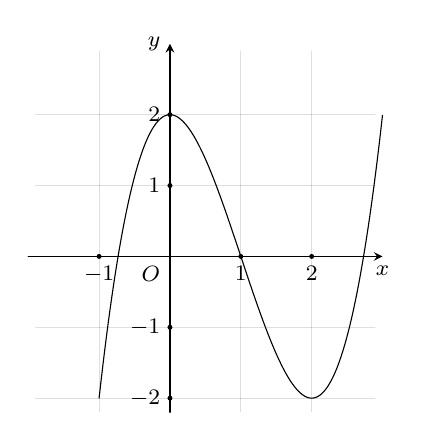
\begin{tikzpicture}[scale=0.9,font=\footnotesize,line join=round,line cap=round,>=stealth]
		\fill (-1.9,-2.2) grid (2.9,2.9); 
		 \draw[->] (-2,0)--(3,0) node[below] {$x$};
		\draw[->] (0,-2.2)--(0,3) node[left] {$y$}; 
		\draw  (0,0) node [below left] {$O$};
		\foreach \x in {-1,1,2} \fill (\x,0) circle (1pt) node [below]  {$\x$};
		\foreach \y in {-2,-1,1,2}  \fill (0,\y) circle (1pt) node [left] {$\y$};
		\draw[smooth,samples=200] plot[domain=-1:3] (\x,{(\x+1)*(\x-2)^2-2}); 
	\end{tikzpicture}
	 }
	\shortans{14} 
	 \loigiai{
		Xét  hàm số $g(x)=f(x-m)-\dfrac{1}{2}(x-m-1)^2+2025$.\\
		Ta  có $g'(x)=f'(x-m)-(x-m-1)$.\\
		Xét phương trình $g'(x)=0(1)$.\\ 
		Đặt $x-m=t$, phương trình $(1)$  trở thành $f'(t)-(t-1)=0\Leftrightarrow f'(t)=t-1$ $(2)$.\\
		Nghiệm của phương trình $(2)$ là hoành độ  giao điểm của hai đồ thị hàm số $y=f'(t)$ và $y=t-1$.\\
		Ta có đồ thị các hàm số $y=f'(t)$ và  $y=t-1$ như sau:
		\begin{center}
			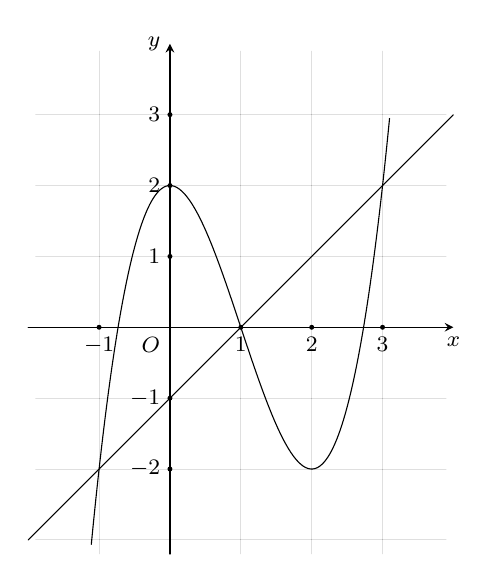
\begin{tikzpicture}[scale=0.9,font=\footnotesize,line join=round,line cap=round,>=stealth]
				\fill (-1.9,-3.2)  grid (3.9,3.9);
				\draw[->] (-2,0)--(4,0) node[below] {$x$}; 
				\draw[->] (0,-3.2)--(0,4) node[left]  {$y$};
				 \draw (0,0) node [below left] {$O$};
				\foreach \x in {-1,1,2,3} \fill (\x,0) circle (1pt)  node [below] {$\x$};
				\foreach \y in {-2,-1,1,2,3} \fill (0,\y) circle (1pt) node  [left] {$\y$};
				 \draw[smooth,samples=200] plot[domain=-1.11:3.1] (\x,{(\x+1)*(\x-2)^2-2});
				 \draw[smooth,samples=200] plot[domain=-2:4] (\x,{(\x)-1});
			\end{tikzpicture}
		\end{center}
		Căn cứ đồ thị các hàm số ta có phương trình  $(2)$ có nghiệm là $\hoac{&t=-1\\
		&t=1\\ 
		&t=3}  \Rightarrow\hoac{&x=m-1\\
		 &x=m+1\\
		&x=m+3.}$ 
		Ta có  bảng biến thiên của $y=g(x)$.
		\begin{center}
			\begin{tikzpicture}[scale=0.9,font=\footnotesize,line join=round,line cap=round,>=stealth]
				 \tkzTabInit
					{$x$/1,$y' $/1,$y$/3} 
					 {$-\infty$,$m-1$,$m+1$,$m+3$,$+\infty$}
				 \tkzTabLine{,-,0,+,0,-,0,+,}
				 \tkzTabVar{+/$+\infty$,-/$0$,+/$3$,-/,+/$+\infty$}
			\end{tikzpicture}
		\end{center}
		Để hàm số $y=g(x)$ đồng biến trên khoảng $(5; 6)$  cần $\hoac{&\heva{&m-1\leq 5\\&m+1\geq 6} \\&m \leq 2}
		 \Leftrightarrow
		\hoac{&5\leq m \leq 6\\&m+3\leq 5.}$\\ 
		Vì  $m \in \mathbb{N}^{*} \Rightarrow m\in \{1;2;5;6\}$. \\
		Tổng các giá trị là $1+2+5+6=14$. 
	 }
\end{bt}

% nguồn: Phan2_Lop_12_Dai_so_Chuong_1
\begin{bt}%[2D1C1-3]%[ma:8b589d80]
	Có bao nhiêu giá  trị nguyên của tham số $m$ để hàm số $y=x^3-3(m+2)x^2+3(m^2+4m)x+1$ nghịch biến trên khoảng $(0; 1)$?
	 \shortans{4}
	 \loigiai{
		Ta có $y'=  3x^2-6(m+2)x+3(m^2+4m)$.\\
		Hàm số nghịch biến trên $(0; 1)$ khi  và chỉ khi
		\begin{eqnarray*}
			y'\leq 0, \forall x\in (0;  1)&\Leftrightarrow& 3x^2-6(m+2)x+3(m^2+4m)\leq 0,\quad \forall x\in (0; 1)\\
			&\Leftrightarrow&(x-m)(3x-3m-12)\leq 0,\quad  \forall x\in (0; 1)\\
			 &\Leftrightarrow& m\leq x\leq m+4,\quad \forall x\in (0; 1)\\
			 &\Leftrightarrow&\heva{&m\leq 0\\&1\leq m+4}\Leftrightarrow -3\leq m\leq 0.
		\end{eqnarray*}
		Vì $m\in\mathbb{Z}$ nên $m \in \{-3; -2; -1; 0\}$.\\ 
		Vậy có $4$ giá trị nguyên $m$ thỏa mãn yêu cầu đề  bài.
	} 
\end{bt}


%%%%%%%%%%%%%%%% TỰ LUẬN %%%%%%%%%%%%%%%%

% nguồn: Phan2_Lop_12_Dai_so_Chuong_1
\begin{bt}%[2D1H1-3]%[ma:af5ca874]
	Tìm tất cả các  giá trị của tham số $m$ để hàm số
	\begin{enumerate}
		\item $y=\dfrac{2x^2+3x+m+1}{x+1}$ đồng biến trên các  khoảng xác định.
		\item $y=\dfrac{x^2+\left(m+1\right)x-1}{2-x}$ ($m$ là tham số) nghịch biến  trên từng khoảng xác định.
	\end{enumerate}
	\loigiai{ 
		\begin{enumerate}
			\item 
			Tập xác định  $\mathscr{D}=\mathbb{R}\setminus \left\{-1\right\}$.\\
			Ta có  $y'=\dfrac{2x^2+4x+2-m}{\left(x+1\right)^2}$.\\
			 Hàm số
			$y=\dfrac{2x^2+3x+m+1}{x+1}$ đồng biến trên  các khoảng xác định khi $y'\ge 0,\,\forall x\in \mathscr{D}$
			\begin{eqnarray*}
				&\Leftrightarrow & 2x^2+4x+2-m\ge 0,\, \forall x\in  \mathbb{R}\\
				&\Leftrightarrow& \Delta'=4-2(2-m)\le 0\\ 
				&\Leftrightarrow  & m\le 0.
			\end{eqnarray*}
			\item Tập xác định $\mathscr{D}=\mathbb{R}\setminus \left\{2\right\}$.\\ 
			Ta có $y'=\dfrac{-x^2+4x+2m+1}{\left(2-x\right)^2}=\dfrac{g(x)}{\left(2-x\right)^2}$  .\\
			Hàm số $y=\dfrac{x^2+\left(m+1\right)x-1}{2-x}$ nghịch biến trên từng khoảng xác định khi $y'\le 0,\,\forall x\in  \mathscr{D}$
			\begin{eqnarray*}
				&\Leftrightarrow& -x^2+4x+2m+1 \le 0 \,\,  \forall x\in \mathbb{R}\\
				 &\Leftrightarrow& \Delta'=4-\left(-1\right)\left(2m+1\right)\le 0\\
				&\Leftrightarrow& 2m+5\le  0\\
				&\Leftrightarrow& m\le-\dfrac{5}{2}. 
			\end{eqnarray*}
		\end{enumerate}
	} 
\end{bt}

% nguồn: Phan2_Lop_12_Dai_so_Chuong_1
\begin{bt}%[2D1H1-3]%[ma:20addd41]
	Tìm tất cả các giá trị của tham số  $m$ để hàm số
	\begin{enumerate}
		\item $y=\dfrac{mx+2}{x+1}$ đồng biến trên  từng khoảng xác định.
		\item $y=\dfrac{mx-2}{x+m-3}$ nghịch biến  trên từng khoảng xác định.
		\item $y=\dfrac{2x+4}{m-x}$ đồng biến  trên $\left(1\,;\,+\infty\right)$.
		\item $y=\dfrac{x+7}{2x+m}$ nghịch biến trên  $\left(-2;+\infty\right)$.
		\item $y=\dfrac{x+m^2-6}{x-m}$ đồng biến trên  khoảng $\left(-\infty;-2\right)$.
		\item $y=\dfrac{x-9}{x+3m}$  đồng biến trên khoảng $\left(-\infty;-6\right)$.
		\item  $y=\dfrac{mx-4}{m-x}$ nghịch biến trên khoảng $\left(-3\,;\,1\right)$.
		\item $y=\dfrac{m^2x+5}{2mx+1}$ nghịch biến  trên khoảng $\left(3;+\infty\right)$.
	\end{enumerate}
	\loigiai{ 
		\begin{enumerate}
			\item  Tập xác định $\mathscr{D}=\mathbb{R}\setminus \{-1\}$.\\
			Ta có $y'=\dfrac{m-2}{(x+1)^2}$.\\ 
			 Hàm đồng biến trên từng khoảng xác định khi \[y' > 0,\,\, \forall x\in \mathscr{D}\Leftrightarrow m-2 > 0\Leftrightarrow m > 2.\]
			\item Tập xác  định $\mathscr{D}=\mathbb{R}\setminus \{3-m\}$.\\
			 Ta có $y'=\dfrac{m^2-3m+2}{\left(x+m-3\right)^2}$.\\
			Hàm  số nghịch biến trên khoảng xác định của nó khi và chỉ khi
			\[y' < 0,\,\forall x\in  \mathscr{D}\Leftrightarrow m^2-3m+2 < 0\Leftrightarrow 1 < m < 2.\]
			\item 
			Tập  xác định $\mathscr{D}=\mathbb{R}\setminus \{m\}$.\\
			Ta có  $y'=\dfrac{2m+4}{(m-x)^2}$.\\
			Để hàm số $y=\dfrac{2x+4}{m-x}$ đồng biến trên $\left(1;\,+\infty\right)$ thì $y' > 0$ với $\forall  x\in\left(1;\,+\infty\right)$.
			 \[\Leftrightarrow \heva{&2m+4>0 \\&m\le 1}\Leftrightarrow -2<m\le 1.\]
			\item 
			Tập xác định $\mathscr{D}=\mathbb{R}\setminus \left\{-\dfrac{m}{2}\right\}$.\\ 
			 Ta có $y'=\dfrac{m-14}{(2x+m)^2}$.\\
			Hàm  số $y=\dfrac{x+7}{2x+m}$ nghịch biến trên $\left(-2;+\infty\right)$ khi $y'<0,\,\forall x\in (-2; +\infty)$
			\[\Leftrightarrow  \heva{&m-14 < 0\\&
			\dfrac{-m}{2}\le-2}\Leftrightarrow \heva{&m\ge 4\\& 
			 m < 14} \Leftrightarrow 4\le m < 14.\]
			 \item
			Tập xác định  $\mathscr{D}=\mathbb{R}\setminus \left\{m\right\}$.\\
			Ta có $y'=\dfrac{-m^2-m+6}{(x-m)^2}$.\\ 
			Hàm số $y=\dfrac{x+m^2-6}{x-m}$ đồng biến  trên khoảng $\left(-\infty;-2\right)$ khi $y'>0,\,\forall x\in (-\infty; -2)$
			\[\Leftrightarrow \heva{&-m^2-m+6>0 \\&m\ge -2}\Leftrightarrow \heva{&-3  < m < 2\\&
			m\ge-2}\Leftrightarrow -2\le m < 2.\] 
			\item 
			Tập xác định  $\mathscr{D}=\mathbb{R}\setminus \left\{-3m\right\}$.\\
			Ta có  $y'=\dfrac{3m+9}{(x+3m)^2}$.\\
			Hàm số $y=\dfrac{x-9}{x+3m}$  đồng biến trên $\left(-\infty;-6\right)$ khi khi $y'>0,\,\forall x\in (-\infty; -6)$
			\[\Leftrightarrow \heva{&3m+9 > 0\\& 
			-6\le-3m}\Leftrightarrow \heva{&m >-3\\& 
			m\le 2}\Leftrightarrow -3 <  m\le 2.\]
			 \item
			Tập  xác định $\mathscr{D}=\mathbb{R}\setminus \left\{m\right\}$.\\
			Ta  có $y'=\dfrac{m^2-4}{\left(m-x\right)^2}$.\\
			Hàm  số $y=\dfrac{mx-4}{m-x}$ nghịch biến trên khoảng $\left(-3\,;\,1\right)$ thì $y'<0,\,\forall x\in (-3; 1)$
			\[\Leftrightarrow \heva{& m^2-4 < 0 \\&m\notin (-3; 1)}\Leftrightarrow\heva{&-2 < m < 2  \\&\hoac{&m\le-3\\&
			m\ge 1} }\Leftrightarrow 1\le m <  2.\]
			\item  Ta xét hai trường hợp sau
			\begin{itemize}
				\item {\bf TH1.} Xét $m=0\Rightarrow y=5$ là  hàm hằng nên hàm số không nghịch biến.\\
				Vậy  $m=0$ không thỏa mãn.\\
				\item {\bf TH2.}  Xét $m\ne 0$.\\
				Tập  xác định $\mathscr{D}=\left(-\infty;\dfrac{-1}{2m}\right)\cup\left(\dfrac{-1}{2m};+\infty\right)$.\\
				Ta có $y'=\dfrac{m^2-10m}{\left(2mx+1\right)^2}$.\\ 
				Để hàm số $y=\dfrac{m^2x+5}{2mx+1}$ nghịch biến trên khoảng  $\left(3;+\infty\right)$ thì $y'>0,\,\forall x\in \left(3;+\infty\right)$
				\[\Leftrightarrow \heva{&{m^2}-10m < 0 \\&\dfrac{-1}{2m}\le 3}\Leftrightarrow \heva{&0 < m < 10 \\&\dfrac{6m+1}{2m}\ge 0}\Leftrightarrow 0  < m < 10.\]
			\end{itemize}
		\end{enumerate}
	 }
\end{bt}
